\title{Architectural Views}
\author{Richard Thomas \& Brae Webb}
\date{\week{2}} % maybe week one?

\maketitle

\section{Introduction}

Understanding software is hard.
It is often claimed that reading code is harder than writing code\footnote{Though evidence suggests that an ability to read and reason 
about code is necessary to learn how to program well \cite{lister-tracing-explaining-writing} \cite{lister-neo-piagetian}.}.
This principle is used to explain a programmers' innate desire to constantly rewrite their code from scratch.
If software is hard to understand, then software architecture is near impossible.
Fortunately, architects have developed a number of techniques to manage this complexity.

A software architecture consists of many dimensions.
Programming languages, communication protocols, the operating systems and hardware used, virtualisation used,
and the code itself are a subset of the many dimensions which comprise a software architecture.
Asking a programmer's monkey brain to understand, communicate, or document every dimension at once is needlessly cruel.
This is where architectural views come in.

Architectural views, or architectural projections, are a representation of one or more related aspects of a software architecture.
Views allow us to focus on a particular slice of our multi-dimensional software architecture, ignoring other irrelevant slices.
For example, if we are interested in applying a security patch to our software then we are only interested in the view
which tells us which software packages are used on each host machine.

The successful implementation of any architecture relies on the ability for the architectural views
to be disseminated, understood, and implemented.
For some organisations, the software is simple enough, or the team small enough, that the design
can be communicated through word of mouth.
As software becomes increasingly complex and developers number in the thousands,
it is critical for design to be communicated as effectively as possible.
In addition to facilitating communication,
architectural views also enable architectural policies to be designed and implemented.

\section{4+1 Views}
Philippe Kruchten was one of the earliest to advocate the idea of using views to design and document software architectures.
In ``4+1 View Model of Software Architecture'' \cite{4+1-model} he describes five different views.
These are logical, process, development, physical, and scenario views, which are summarised below.
\begin{description}
    \item[Logical] How functionality is implemented, using class and state diagrams.
    \item[Process] Runtime behaviour, including concurrency, distribution, performance and scalability.
                            Sequence, communication and activity diagrams are used to describe this view.
    \item[Development] The software structure from a developer's perspective, using package and component diagrams.
                                    This is also known as the implementation view.
    \item[Physical] The hardware environment and deployment of software components.
                            This is also known as the deployment view.
    \item[Scenario] The key usage scenarios that demonstrate how the architecture delivers the functional requirements.
                             This is the `+1' view as it is used to validate the software architecture.
                             This is also known as the use case view, as high-level use case diagrams are used to outline the key use cases and actors.
\end{description}
The experience which led to the development the 4+1 View Model was developing the air traffic control management system for Canada.
The system provides an integrated air traffic control system for the entire Canadian airspace.
This airspace is about double the size of the Australian airspace and borders the two busiest airspaces in the world.
The project's architecture was designed by a team of three people led by Philippe.
Development was done by a team of 2500 developers from two large consulting companies.
The project was delivered on-time and on-budget, with three incremental releases in less than three years\footnote{Contrast
this to the United States Federal Aviation Administration's Advanced Automation System project from a similar era.
The original estimate was \$2.5 billion and fourteen years to implement.
The project was effectively cancelled after twelve years.
By then the estimate had almost tripled and the project was at least a decade behind schedule \cite{faa-aas}.}.
This project also developed many of the ideas that led to the Rational Unified Process \cite{kruchten2004rational}.

\section{\textit{Software Architecture in Practice} Views}
The seminal architecture book, \textit{Software Architecture in Practice} \cite{bass2021software},
categorises architectural views into three groups.
These three groups each answer different questions about the architecture, specifically:
\begin{description}
    \item[Module Views] How implementation components of a system are structured and depended upon.
    \item[Component-and-connector Views] How individual components communicate with each other.
    \item[Allocation Views] How the components are allocated to personnel, file stores, hardware, etc.
\end{description}

\subsection{Module Views}
Module views are composed of modules, which are static units of functionality such as classes, functions, packages, or whole programs.
The defining characteristic of a module is that it represents software responsible for some well-defined functionality.
For example, a class which converts JSON to XML would be considered a module, as would a function which performs the same task.

The primary function of module views is to communicate the dependencies of a module.
Rarely does software work completely in isolation, often it is constructed with implicit or explicit dependencies.
A module which converts JSON to XML might depend upon a module which parses JSON and a module which can format XML.
Module views make these dependencies explicit.

Module views focus on the developer's perspective of how the software is implemented, rather than how it manifests itself when deployed in a computing environment.

\begin{figure}[ht]
\centering
\begin{subfigure}[b]{\textwidth}
\begin{shaded}
\begin{lstlisting}[style=python]
import json
import xml

class JSONtoXML:
    def load(self, json_file):
        with open(json_file) as f:
            data = json.load(f)
        self.data = self.convert(data)

    def export(self, xml_file):
        xml.write(xml_file, data)

    def convert(self, data: JSON) -> XML:
        ...
\end{lstlisting}
\end{shaded}
\caption{Pseudo-code to convert JSON to XML}
\end{subfigure}


\begin{subfigure}[b]{\textwidth}
\begin{center}
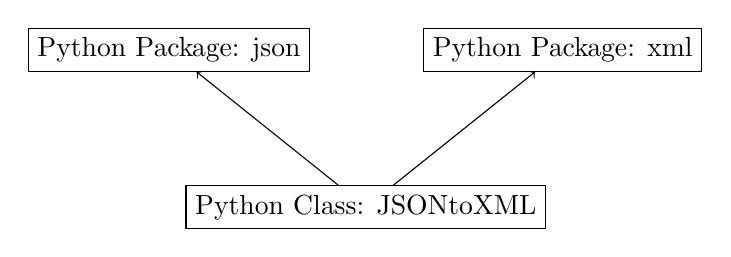
\begin{tikzpicture}
    \node[draw] (json) at (0,0) {Python Package: json};
    \node[draw] (xml) at (5,0) {Python Package: xml};
    \node[draw] (jsontoxml) at (2.5,-2) {Python Class: JSONtoXML};

    \path [->] (jsontoxml) edge node {} (json);
    \path [->] (jsontoxml) edge node {} (xml);
\end{tikzpicture}
\end{center}
\caption{An example of a module view which illustrates the dependencies of the \texttt{JSONtoXML} class}
\end{subfigure}
\caption{A simple module view of a JSON to XML program.}
\end{figure}

\subsection{Component-and-Connector Views}
Component-and-connector views focus on the structures that deliver the runtime, or dynamic behaviour of a system.
Components are units which perform some computation or operation at runtime.
These components could overlap with the modules of a module view but are often at a higher level of abstraction.
The focus of component-and-connector views is how these components communicate at runtime.
Runtime communication is the connector of components.
For example, a service which registers users to a website might have new registrations communicated via a \link{REST}{https://www.ibm.com/cloud/learn/rest-apis} request.
The service may then communicate the new user information to a database via SQL queries.

When we look at software architecture, component-and-connector views are the most commonly used views.
They are common because they contain runtime information which is not easily automatically extracted.
Module views can be generated after the fact, i.e. it is easy enough for a project to generate a UML class diagram.
(Simple tools will create an unreadably complex class diagram.
Tagging important information in the source code, or manually removing small details is required to end up with readable diagrams.)
Component-and-connector views are often maintained manually by architects and developers.

\subsection{Allocation Views}
According to Bass et al, allocation views map the software's structures to the system's non-software structures \cite{bass2021software}.
They include concepts such as who is developing which software elements,
where are source files stored for different activities such as development and testing,
and where are software elements executed.
The first two points are important for project management and build management.
The last point of how the software is executed on different processing nodes is important for architectural design.
This is sometimes called the \emph{deployment structure} or the software system's \emph{physical architecture}.

Understanding the physical architecture (simplistically the hardware\footnote{Whether it is virtualised or physical hardware}
on which the software is executed) is important when designing the software's \emph{logical architecture}.
Component-and-connector views describe the software's logical architecture.
This design of the logical architecture must contain components that can be allocated appropriately to processing nodes,
and these nodes must have communication links that enable the components to interact.

\section{Sahara eCommerce Example}\label{sec:storeExample}
Sahara\footnote{Yes, that is intentionally a dry joke.} eCommerce is an ambitious company who's prime business unit is an on-line store selling a wide range of products.
They provide both web and mobile applications to deliver the shopping experience to customers.

\subsection{Architecturally Significant Requirements}\label{sec:storeReq}
\emph{Architecturally significant requirements} (ASR) are functional or non-functional requirements,
or constraints or principles, which influence the design of the system architecture.
The structure of a software architecture has to be designed to ensure that the ASRs can be delivered.

Not all requirements for a system will be architecturally significant, but those that are need to be identified.
Once ASRs are identified, an architecture needs to be designed to deliver them.
This may require some research, and experimentation with prototypes, to determine which options are appropriate.
Tests should be designed to verify that the architecture is delivering the ASRs.
Ideally, these should be part of an automated test suite.
This may not be possible for all tests.
Regardless, the ASR tests should be executed frequently during development to provide assurance that the system will deliver the ASRs.

Inevitably, some ASRs will be discovered later in the project.
The existing architecture will need to be evaluated to determine if it can deliver the new ASRs.
If it can, new tests need to be added to the ASR test suite to verify delivery of the new ASRs.
If the architecture is no longer suitable due to the new ASRs,
a major redesign needs to be done to create a new, more suitable, architecture.

The architecturally significant requirements for the Sahara eCommerce system are:
\begin{itemize}
    \item Customers can start shopping on one device and continue on another device.
             (e.g. Add a product to their shopping cart while browsing on their computer when they are bored at school.
              Checkout their shopping cart from their mobile phone on their way home on the bus.)
    \item The system must be scalable. It must cater for peaks in demand (e.g. Cyber Monday and Singles Day).
             It must cater for an unknown distribution of customers accessing the on-line store through web or mobile applications.
    \item The system must be robust. The system must continue to operate if a server fails.
             It must be able to recover quickly from sub-system failures.
    \item The system must have high availability.
             Target availability is ``four nines''\footnote{A number of nines (e.g. four nines)
             is a common way to measure availability. It represents the percentage of time the system is ``up''.
             Four nines means the system is available 99.99\% of the time, or it is not available for less than one hour per year.}
            up time.
\end{itemize}
\noindent
The following sections will describe the physical and software architecture for this system, and demonstrate how it delivers these ASRs.

\subsection{Allocation View}\label{sec:storeAllocView}
Figure \ref{fig:deploymentDiagram} uses a UML deployment diagram as a visual representation of the physical architecture of the system as part of the allocation view.
The diagram also shows some of the important software components that are deployed onto parts of the physical architecture.
For simplicity, details such as load balancing and failover are not shown in this example.

\begin{figure}[h!]
    \centering
    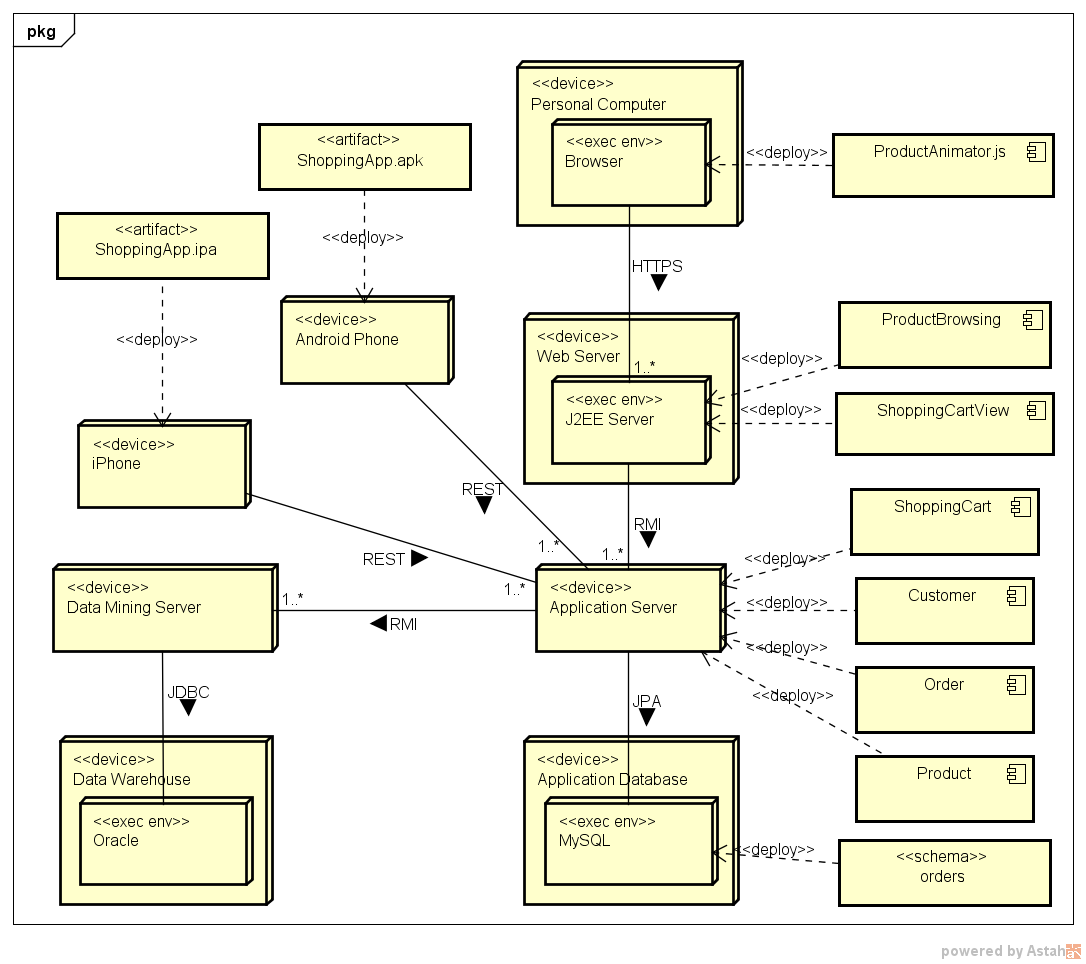
\includegraphics[trim=38 38 23 44,clip,width=0.92\textwidth]{images/uml/deployment_diagram.png}
    \caption{Example physical architecture for the Sahara eCommerce system.}
    \label{fig:deploymentDiagram}
\end{figure}

There are both web and mobile applications that customers use to shop at the store.
A J2EE server (e.g. \link{TomEE}{https://tomee.apache.org/}), running on a web server hardware platform,
handles browser requests from customers, using the HTTPS protocol over the Internet.
A JavaScript module called \texttt{ProductAnimator} is downloaded to the customer's browser to allow them to see interactive 3d views of products.
The \texttt{ProductBrowsing} and \texttt{ShoppingCartView} components run on the J2EE server, providing those aspects of the user interaction.
The J2EE server uses RMI\footnote{Remote Method Invocation} over a network connection to an application server.

The application server provides the shared logic of the on-line store.
This supports implementing the functional requirement that a customer can start shopping on one device and continue on another.
Running the applicaiton server on its own device allows easier scalability of the system.
The application server could be replicated on multiple devices to handle requests from different sources, without duplicating unneeded web or database logic.
Examples of components that would run on the application server are \texttt{Customer}, \texttt{ShoppingCart}, \texttt{Order} and \texttt{Product}.

The application server uses JPA\footnote{Java Persistence API} over a network connection to communicate with the application data\-base running on a separate server.
The \texttt{orders} schema is an example of one of the tables that would be created in the application database.
The application server also uses RMI over a network connection to communicate with a data mining server.

The data mining server uses JDBC\footnote{Java DataBase Connectivity} over a network connection to a server running the data warehouse.
The mobile applications run on their respective phone environments and use REST API calls over the Internet to interact with application server.

\textbf{Note}, for web applications the customer's computer and browser would only be shown in the deployment diagram
if the software system downloads application logic that executes in the browser (e.g. JavaScript).
In this example the \texttt{ProductAnimator.js} module is an important part of the application's functional requirements.

\subsubsection{Deployment Diagram Notation}\label{sec:deploymentNotation}
In the diagram, cube icons represent \emph{nodes}. Nodes are computational resources that can execute software artifacts.
Nodes may be \guillemotleft device\guillemotright's, representing hardware.
They may also be \guillemotleft executionEnvironment\guillemotright's, representing software that provides an environment in which other software artifacts can be executed.
(The keyword has been shortened to \guillemotleft exec env\guillemotright~in this example.)
Execution environments need to be allocated to devices.
In figure \ref{fig:deploymentDiagram}, \texttt{Browser} and \texttt{J2EE Server} are software environments running,
respectively, on the hardware devices \texttt{Personal Computer} and \texttt{Web Server}.

The solid lines between nodes are \emph{associations}, which represent communication paths.
A communication path can represent a \emph{physical connection} or \emph{protocol}.
Formally, a stereotype (e.g. \guillemotleft protocol\guillemotright) is used to distinguish the type of communication path.
In figure \ref{fig:deploymentDiagram}, all communication paths are protocols so the stereotype is not included.
The protocol name is used to indicate which one is being used on the communication path.
The end of an association can indicate \emph{multiplicity}.
In a deployment diagram this is used to indicate that some nodes may be replicated
(e.g. for performance or robustness). The `*' symbol is used to indicate many instances may be involved.

The rectangles with a `plug' icon in their top-right corner are \emph{components}.
Components are executable software which need to be deployed to a node on which they will run.
The dashed dependency arrow, with the stereotype \guillemotleft deploy\guillemotright, indicates the node on which the component will be deployed for execution.

\textbf{Note}, this approach of showing components being deployed to nodes is an older style of UML.
The current version of UML has the concept of \emph{artifacts} being deployed to nodes.
Artifacts can implement (manifest in UML terminology) components, which provides an additional layer of abstraction.
Formally, components would be manifested by an artifact that is then deployed to a node.
In figure \ref{fig:deploymentDiagram}, components are deployed directly to nodes to keep the diagram simple.
UML provides multiple ways to indicate which artifacts are deployed on a node, e.g. a textual list of artifacts inside the node icon.
The approach taken for a diagram should be chosen to aid readability and reduce clutter.

Artifacts are used in this diagram to represent software that has to be packaged
(i.e. deployed through a manifest), which corresponds to the idea of an artifact in the note above.
An artifact is represented by a rectangle with the \guillemotleft artifact\guillemotright~keyword and the name of the artifact that is created for deployment.

The \guillemotleft schema\guillemotright~stereotype indicates that the artifact is a database schema describing tables to be created in the database.

\subsection{Component-and-Connector View}\label{sec:CnC_view}
Figure \ref{fig:componentDiagram} uses a UML component diagram as a visual representation of
the logical components that deliver system behaviour as part of the component-and-connector view.
It models the logical architecture of the components that allow customers to browse for products, add them to their shopping cart, and purchase them.
To keep the example manageable, this is the only part of the system that is shown in this view.

\begin{figure}[h]
    \centering
    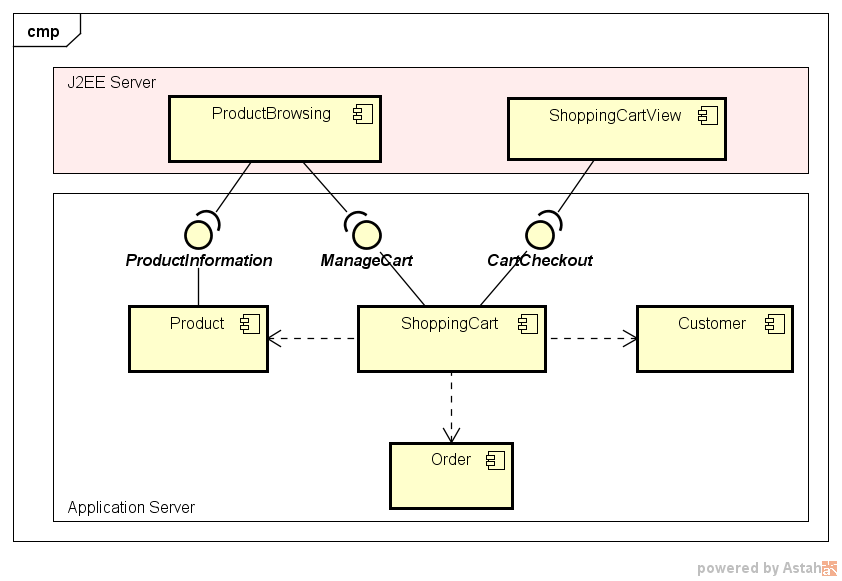
\includegraphics[trim=39 37 22 49,clip,width=0.8\textwidth]{images/uml/component_diagram.png}
    \caption{Example logical architecture -- browsing for products and purchasing them.}
    \label{fig:componentDiagram}
\end{figure}

As was shown in figure \ref{fig:deploymentDiagram},
the \texttt{ProductBrowsing} and \texttt{ShoppingCartView} components are deployed on the J2EE server.
These two component provide the user interaction behaviour in the web application
of browsing for products, adding them to the shopping cart, and purchasing the products.

The \texttt{Product}, \texttt{ShoppingCart}, \texttt{Order} and \texttt{Customer} components are deployed on the application server.
These components deliver the logical behaviour of providing information about products, tracking what is in the shopping cart, and placing orders.

The \texttt{ProductBrowsing} component uses the \texttt{\textsl{ProductInformation}} and \texttt{\textsl{ManageCart}} interfaces.
These two interfaces are realised (or implemented) by the \texttt{Product} and \texttt{ShoppingCart} components respectively.
The \texttt{ShoppingCartView} component uses the \texttt{\textsl{CartCheckout}} interface, which is realised by the \texttt{ShoppingCart} component.
These interfaces describe the communication pathways between the components on the different nodes of the physical architecture.

The \texttt{ShoppingCart} component uses the \texttt{Product}, \texttt{Customer} and \texttt{Order} components.
At the programming level, there could be interfaces between these components which are not shown in this diagram.

\noindent
The applicaiton database is not shown in this component diagram as all of its behaviour is defined within the application server's logic.
JPA automates the process of saving and retrieving objects from a relational database.
Consequently, the database is just a storage mechanism and does not implement any application logic.
If the database implemented logic (e.g. through stored procedures and constraints),
then components representing that logical behaviour would be included in this diagram.

\subsubsection{Component Diagram Notation}\label{sec:componentNotation}
As indicated in \ref{sec:deploymentNotation}, rectangles with the `plug' icon represent \emph{components} in UML.

Circles represent \emph{interfaces}, and are labelled with the interface's name.
A line from a component to an interface circle indicates that the component provides (or realises) the interface.

Cups represent a \emph{required interface}, and a line from a component to a cup indicates that the component depends on (or uses) the interface.
This notation visualises the connection between components.

Dependency arrows point from a component whose runtime behaviour depends on behaviour provided by the target component.

Boxes around groups of components are \emph{system boundary boxes}.
They represent a logical grouping of elements in a UML diagram and can be given a name to describe the grouping.
Colours and shading can be used to help distinguish between different logical groups.

\subsubsection{Behaviour Structure}\label{sec:behaviourStruct}
With complex systems it can be helpful to describe how the behaviour is implemented.
UML sequence and communication diagrams can be used to show this behavioural structure.
Figure \ref{fig:sequenceDiagram} is a high-level sequence diagram describing how the
\texttt{ProductBrowsing} component in the J2EE server collaborates with the
\texttt{ShoppingCart} component on the application server to deliver the behaviour of a customer adding a product to their shopping cart.
It also shows \texttt{ShoppingCart} component communicating with the application database.

\begin{figure}[h!]
    \centering
    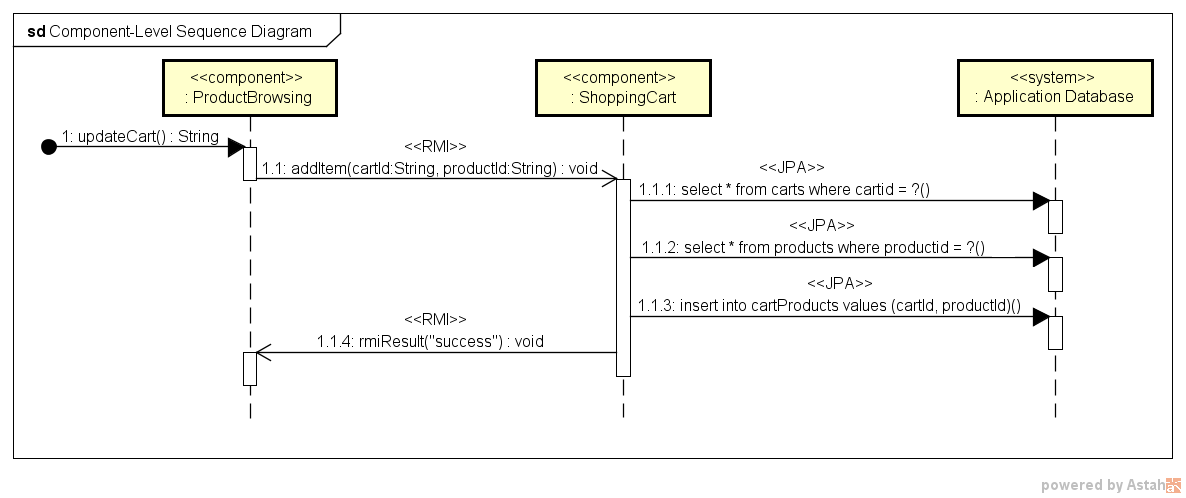
\includegraphics[trim=28 70 23 44,clip,width=\textwidth]{images/uml/component-level_sequence_diagram.png}
    \caption{Example behavioural description -- customer adding a product to their shopping cart.}
    \label{fig:sequenceDiagram}
\end{figure}

Figure \ref{fig:sequenceDiagram} does not provide much additional information that is not already shown or implied by
figures \ref{fig:deploymentDiagram} and \ref{fig:componentDiagram}.
Normally sequence or communication diagrams would be used to describe behaviour that is not clear from other diagrams and descriptions.
This can include complex interactions between modules, complex concurrency, real-time constraints, or latency constraints.

\noindent
For example, when Boeing was upgrading the combat control system of the \link{F-111}{https://www.youtube.com/watch?v=xUcpZJE050s}
for the Australian Airforce, they used a software architecture that used
\link{CORBA}{https://www.ibm.com/docs/en/integration-bus/9.0.0?topic=corba-common-object-request-broker-architecture} as middleware.
The implementation of the middleware caused a fixed delay in sending messages between components.
From an architectural design perspective, it was important to document this delay and enforce a maximum delay on the time taken to complete any process.
A sequence diagram can use constraints to indicate these types of real-time restrictions in your design.

\subsubsection{Sequence Diagram Notation}\label{sec:sequenceNotation}
Sequence diagrams are read from the top down.
The top of the diagram represents the start of the scenario, and execution time progresses down the diagram.
The bottom of the diagram is the end of the scenario.
Duration constraints can be placed between messages indicating information like the maximum allowed time between the start and end of a message.

Rectangles with lines descending from them are \emph{lifelines}.
They represent an instance of a participant in the scenario being described.
The name at the top of a lifeline describes the participant.
In figure \ref{fig:sequenceDiagram}, these are components or the database system.

The horizontal lines are \emph{messages} sent between participants.
Messages use hierarchical numbers to indicate both nesting and sequence of messages.
Message 1.1 is sent by message 1. Message 1.1.1 comes before message 1.1.2.
Message 1 in figure \ref{fig:sequenceDiagram} is a \emph{found message}, meaning that the sender of the message is not shown in the diagram.

A closed arrowhead on a message (e.g. message 1) indicates that it is a synchronous message.
An open arrowhead on a message (e.g. message 1.1) indicates that it is an asynchronous message.
In figure \ref{fig:sequenceDiagram}, stereotypes have been placed on most messages to indicate the protocol used to send the message.

The vertical rectangles sitting on top of lifelines are \emph{execution specifications}.
They indicate when an instance is executing logic.
For example, after the asynchronous message 1.1 is sent to the \texttt{ShoppingCart} component,
message 1 finishes executing.
When the synchronous message 1.1.1 is sent to the database, message 1.1 is still active
as it is waiting for message 1.1.1 to finish before message 1.1 can continue to the next part of the logic.

\subsection{Module View}\label{sec_moduleView}
Figure \ref{fig:classDiagram} uses a UML class diagram as a visual representation of the static structure
of the classes that implement the \texttt{ShoppingCart} component as part of the module view.
Usually only architecturally significant operations and attributes are shown.
(e.g. Operations and attributes needed to understand relationships and behaviour in the component-and-connector view.)
And for simplicity in this diagram, only the classes and interfaces related to adding items to a shopping cart and checking out are shown.

\begin{figure}[h]
    \centering
    \begin{adjustwidth}{-10.5mm}{-11mm}
        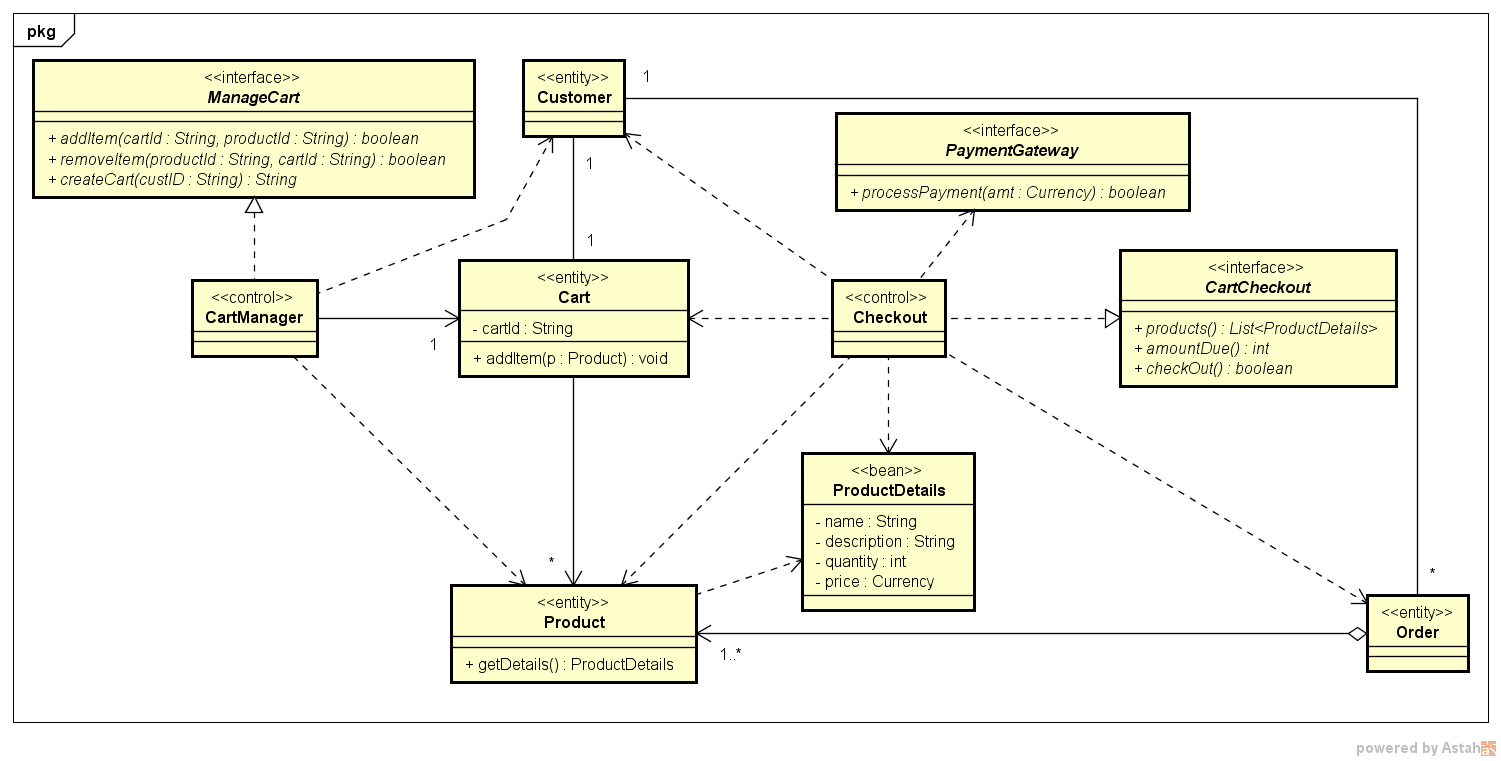
\includegraphics[trim=22 45 22 44,clip,width=0.98\paperwidth]{images/uml/shopping_cart_class_diagram.png}
    \end{adjustwidth}
    \caption{Example static structure for part of the shopping cart package in the class model.}
    \label{fig:classDiagram}
\end{figure}

\noindent
The \texttt{CartManager} and \texttt{Checkout} control classes implement, respectively,
the \texttt{\textsl{ManageCart}} and \texttt{\textsl{Cart\-Check\-out}} interfaces.
These two classes implement the Façade design pattern and manage how
adding products to a shopping cart and checking out are delivered by the classes in this package.
Going back to the component and connector view (figure \ref{fig:componentDiagram}),
when a customer, via their web browser, selects to add a product to their shopping cart,
the \texttt{ProductBrowsing} component's logic uses the \texttt{\textsl{ManageCart}}
interface's \texttt{additem} operation to send a message to the \texttt{ShoppingCart} component.

In the implementation of the \texttt{ShoppingCart} component,
the \texttt{CartManager} class uses the cart and product JPA data access objects (DAOs)
to load the product details and the customer's shopping cart from the application database.
The DAOs create \texttt{Product} and \texttt{Cart} entity objects, and \texttt{CartManager} adds the product to the cart.
Once this is done the \texttt{CartDAO} is used to save the updated cart data into the database.

When a customer wants to checkout the products in their shopping cart, the \texttt{ShoppingCartView} component
uses the \texttt{\textsl{Checkout}} interface's \texttt{products} operation to get a list of the product details to be displayed in the shopping cart.
The \texttt{ProductDetails} class is a Java bean that is used to pass the data about each product to the \texttt{ShoppingCartView}.
Once a customer decides to buy the products in their shopping cart,
the \texttt{ShoppingCartView} sends the \texttt{checkOut} message to the \texttt{ShoppingCart}.
\texttt{Checkout} uses the \texttt{\textsl{PaymentGateway}} interface to process the payment.

\subsubsection{Class Diagram Notation}\label{sec:classNotation}
Formally in UML, rectangles represent \emph{classifiers}. A \emph{class} is one type of classifier.
In a class diagram, a rectangle represents a class, unless a keyword is used to indicate that it is a different type of classifier.
Classifier rectangles have three compartments.
The top compartment contains its name and optionally includes a keyword, stereotypes and properties for the classifier.
The middle compartment contains \emph{attributes}.
The bottom compartment contains \emph{operations}.

Solid lines represent \emph{associations}, which may optionally have an arrow indicating the direction of the relationship.
An association indicates a structural relationship between classes.
Typically this means that the target of an association will be an implicit attribute of the class.
The end of an association can use \emph{multiplicity} to indicate the number of objects of the class that may take part in the relationship.

\noindent
A diamond on the end of an association indicates \emph{aggregate} relationship.
The diamond is on the end that is the aggregate, and the other end is the part.
The diamond may be filled or not. A filled diamond represents \emph{composition} in UML.
This indicates `ownership', where the aggregate controls the lifespan of the part.
A hollow diamond, as in the relationship between \texttt{Order} and \texttt{Product},
indicates \emph{aggregation} in UML.
This is a weaker relationship than composition, as the aggregate does not control the lifespan of the part,
but it still indicates a strong relationship between the classes.

A dashed line with an open arrowhead (e.g. from \texttt{CartManager} to \texttt{Product})
indicates that one classifier \emph{depends} on (or uses) another. This is meant to indicate a transient relationship.

A dashed lines with a closed and hollow arrowhead (e.g. from \texttt{Checkout} to \texttt{\textsl{CartCheckout}})
indicates that the class is \emph{realising} (or implementing) that interface.

\textit{Italicised} names indicate an abstract classifier. Keywords are used to indicate the type of a classifier.
In this example, the keyword \guillemotleft interface\guillemotright~indicates that the classifier is an interface.
Stereotypes use the same notation as keywords. Three standard stereotypes for classes in UML are:
\begin{description}[nosep,left=5mm]
    \item[\guillemotleft entity\guillemotright] Represents a concept (\emph{entity}) from the problem domain.
    \item[\guillemotleft control\guillemotright] Provides logical behaviour from the solution domain.
    \item[\guillemotleft boundary\guillemotright] Communicates with something outside of the system. (Not shown in diagram.)
\end{description}
An additional stereotype \guillemotleft bean\guillemotright~is used to indicate that the class is a Java bean.

\subsubsection{Detailed Behaviour Structure}\label{sec:detailedBehaviourStruct}
Figure \ref{fig:detailedSequenceDiagram} is a detailed sequence showing how the class model in
figure \ref{fig:classDiagram} implements the behaviour of a customer adding a product to their shopping cart.
Like with the high-level sequence diagram, you would only provide detailed sequence diagrams to describe architecturally important details of the design.

\begin{figure}[h!]
    \centering
    \begin{adjustwidth}{-11mm}{-11mm}
        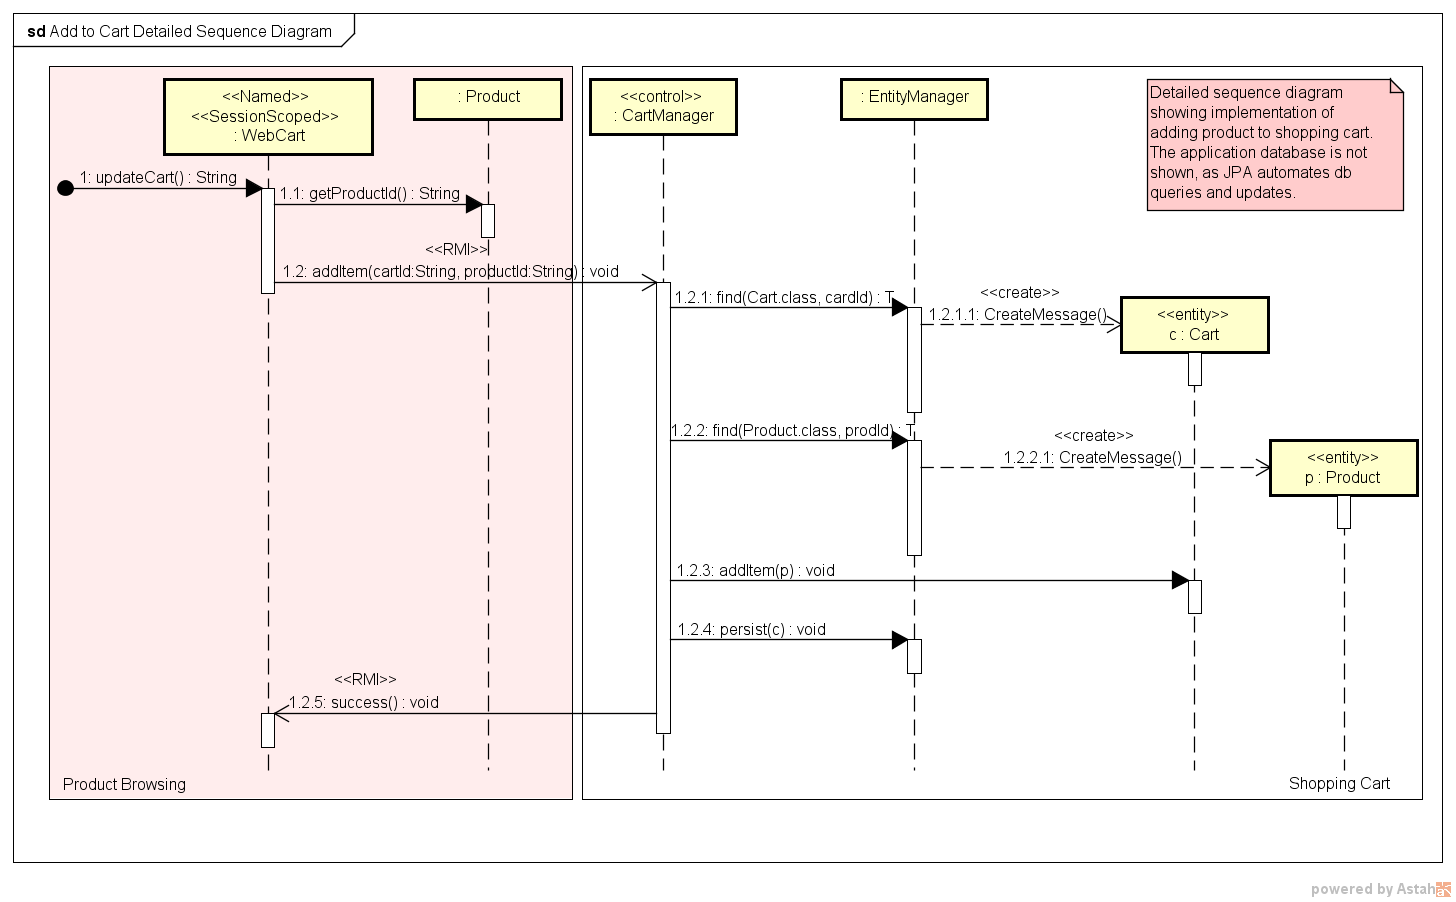
\includegraphics[trim=35 70 31 49,clip,width=0.98\paperwidth]{images/uml/detailed_sequence_diagram.png}
    \end{adjustwidth}
    \caption{Example detailed sequence diagram showing the implementation of customer adding a product to their shopping cart.}
    \label{fig:detailedSequenceDiagram}
\end{figure}

\noindent
The scenario starts with the JSF session-scoped bean \texttt{WebCart} receiving the \texttt{updateCart} message from the browser.
\texttt{WebCart} retrieves the product id and uses the \texttt{ManageCart} interface to send it, along with the cart id,
to the \texttt{ShoppingCart} component on the application server.
The \texttt{ManageCart} interface is implemented by the \texttt{CartManager} class in the \texttt{ShoppingCart} component.

The \texttt{CartManager} uses two JPA data access objects (DAOs) to retrieve the cart and product entities from the application database.
Once the product is added to the cart, the \texttt{CartDAO} saves the updated cart details to the database.
Upon successfully saving the updated cart, the \texttt{CartManager} notifies the \texttt{WebCart}
object in the \texttt{ProductBrowsing} component in the J2EE server.

\subsubsection{Sequence Diagram Notation}
The \guillemotleft create\guillemotright~and \guillemotleft destroy\guillemotright~stereotypes indicate when instances are created or destroyed.
When an instance is created, its lifeline starts at the level of the sequence diagram that indicates the time when it is created.
When an instance is destroyed, its lifeline finishes, with a large \texttt{X}.
Lifelines that are at the top of the diagram indicate instances that existed before the start of the scenario.
Lifelines that reach the bottom of the diagram indicate instances that still exist after the end of the scenario.

In figure \ref{fig:detailedSequenceDiagram}, system boundary boxes are used to indicate which objects execute on which nodes from the deployment diagram.

\subsection{Delivering Architecturally Significant Requirements}
In section \ref{sec:storeReq}, four ASRs were identified for the Sahara eCommerce system.
These were the abililty to continue shopping on different devices, scalability, robustness and availability.

Implementing shared logic on an application server, as shown in figure \ref{fig:deploymentDiagram},
enables the web and mobile applications to share common logic and state.
This delivers the functionality of allowing a customer to start shopping on one device and to continue on another device.
It also minimises duplication of logic, as it is shared by the frontend applications.

Using separate servers for the web server, application server, application database, and data mining server,
as shown in figure \ref{fig:deploymentDiagram}, provides more options to deliver scalability, robustness and availability.
For scalability and performance, each computing environment can be optimised for the services it delivers.
It also means that new servers can be deployed to target specific bottlenecks.

The system follows the \link{\emph{stateless architecture} pattern}{https://www.redhat.com/en/topics/cloud-native-apps/stateful-vs-stateless}.
The web and mobile applications do not store any application state (e.g. products currently stored in the shopping cart).
Every time the customer performs a transaction (e.g. viewing product details or adding a product to their shopping cart),
the web or mobile application sends a message to the application server to perform the action.
The application server then saves or loads data to or from the application database.
This means that web and mobile applications can send messages to a different application server for each request.
This facilitates scalability, robustness and availability.
A new application server can be started to cater for increasing system load, or to replace a failed server.
The stateless nature of the application server logic means that no data will be lost if a server fails,
or if a frontend application accesses a different application server in the middle of a customer's shopping experience.

Having multiple application servers, and multiple application databases and data mining servers,
means that if one server fails its load can be picked up by other servers.
Automating the process of starting or restarting servers improves robustness and availability.

One challenge of a stateless architecture is providing a replicated database that contains up-to-date copies of the system's state.
We will look at this issue later in the course.

By designing the architecture as a set of components running on different servers, it is also easier to migrate the application to cloud-based infrastructure.
Figure \ref{fig:deploymentDiagram} does not constrain the system to run on physical hardware hosted by Sahara eCommerce.
Any of the nodes could be provisioned by a service offered by a cloud provider.
Figure \ref{fig:c4_deployment} in section \ref{sec:c4_deployment} provides an example of a hybrid cloud solution.
In that example, the on-line store components of the architecture run on hardware hosted by Sahara eCommerce.
The data mining components run on Oracle's cloud infrastructure.

\section{C4 Model}
Simon Brown's C4 model provides a set of abstractions that describe the static structure of the software architecture \cite{brown2022c4}.
The C4 model uses these abstractions in a hierarchical set of diagrams, each leading to finer levels of detail.
The hierarchical structure is based on the idea that a software system is composed of containers, which are implemented by components, that are built using code.
\begin{description}
    \item[Software System] Something that delivers functional value to its users (human or other systems).
    \item[Containers] Deployable `block' of code or data that provides behaviour as part of the software system.
    \item[Components] Encapsulate a group of related functionality, usually hidden behind a published interface.
    \item[Code] Elements built from programming language constructs, e.g. classes, interfaces, functions, ....
\end{description}

\begin{figure}[h]
    \centering
    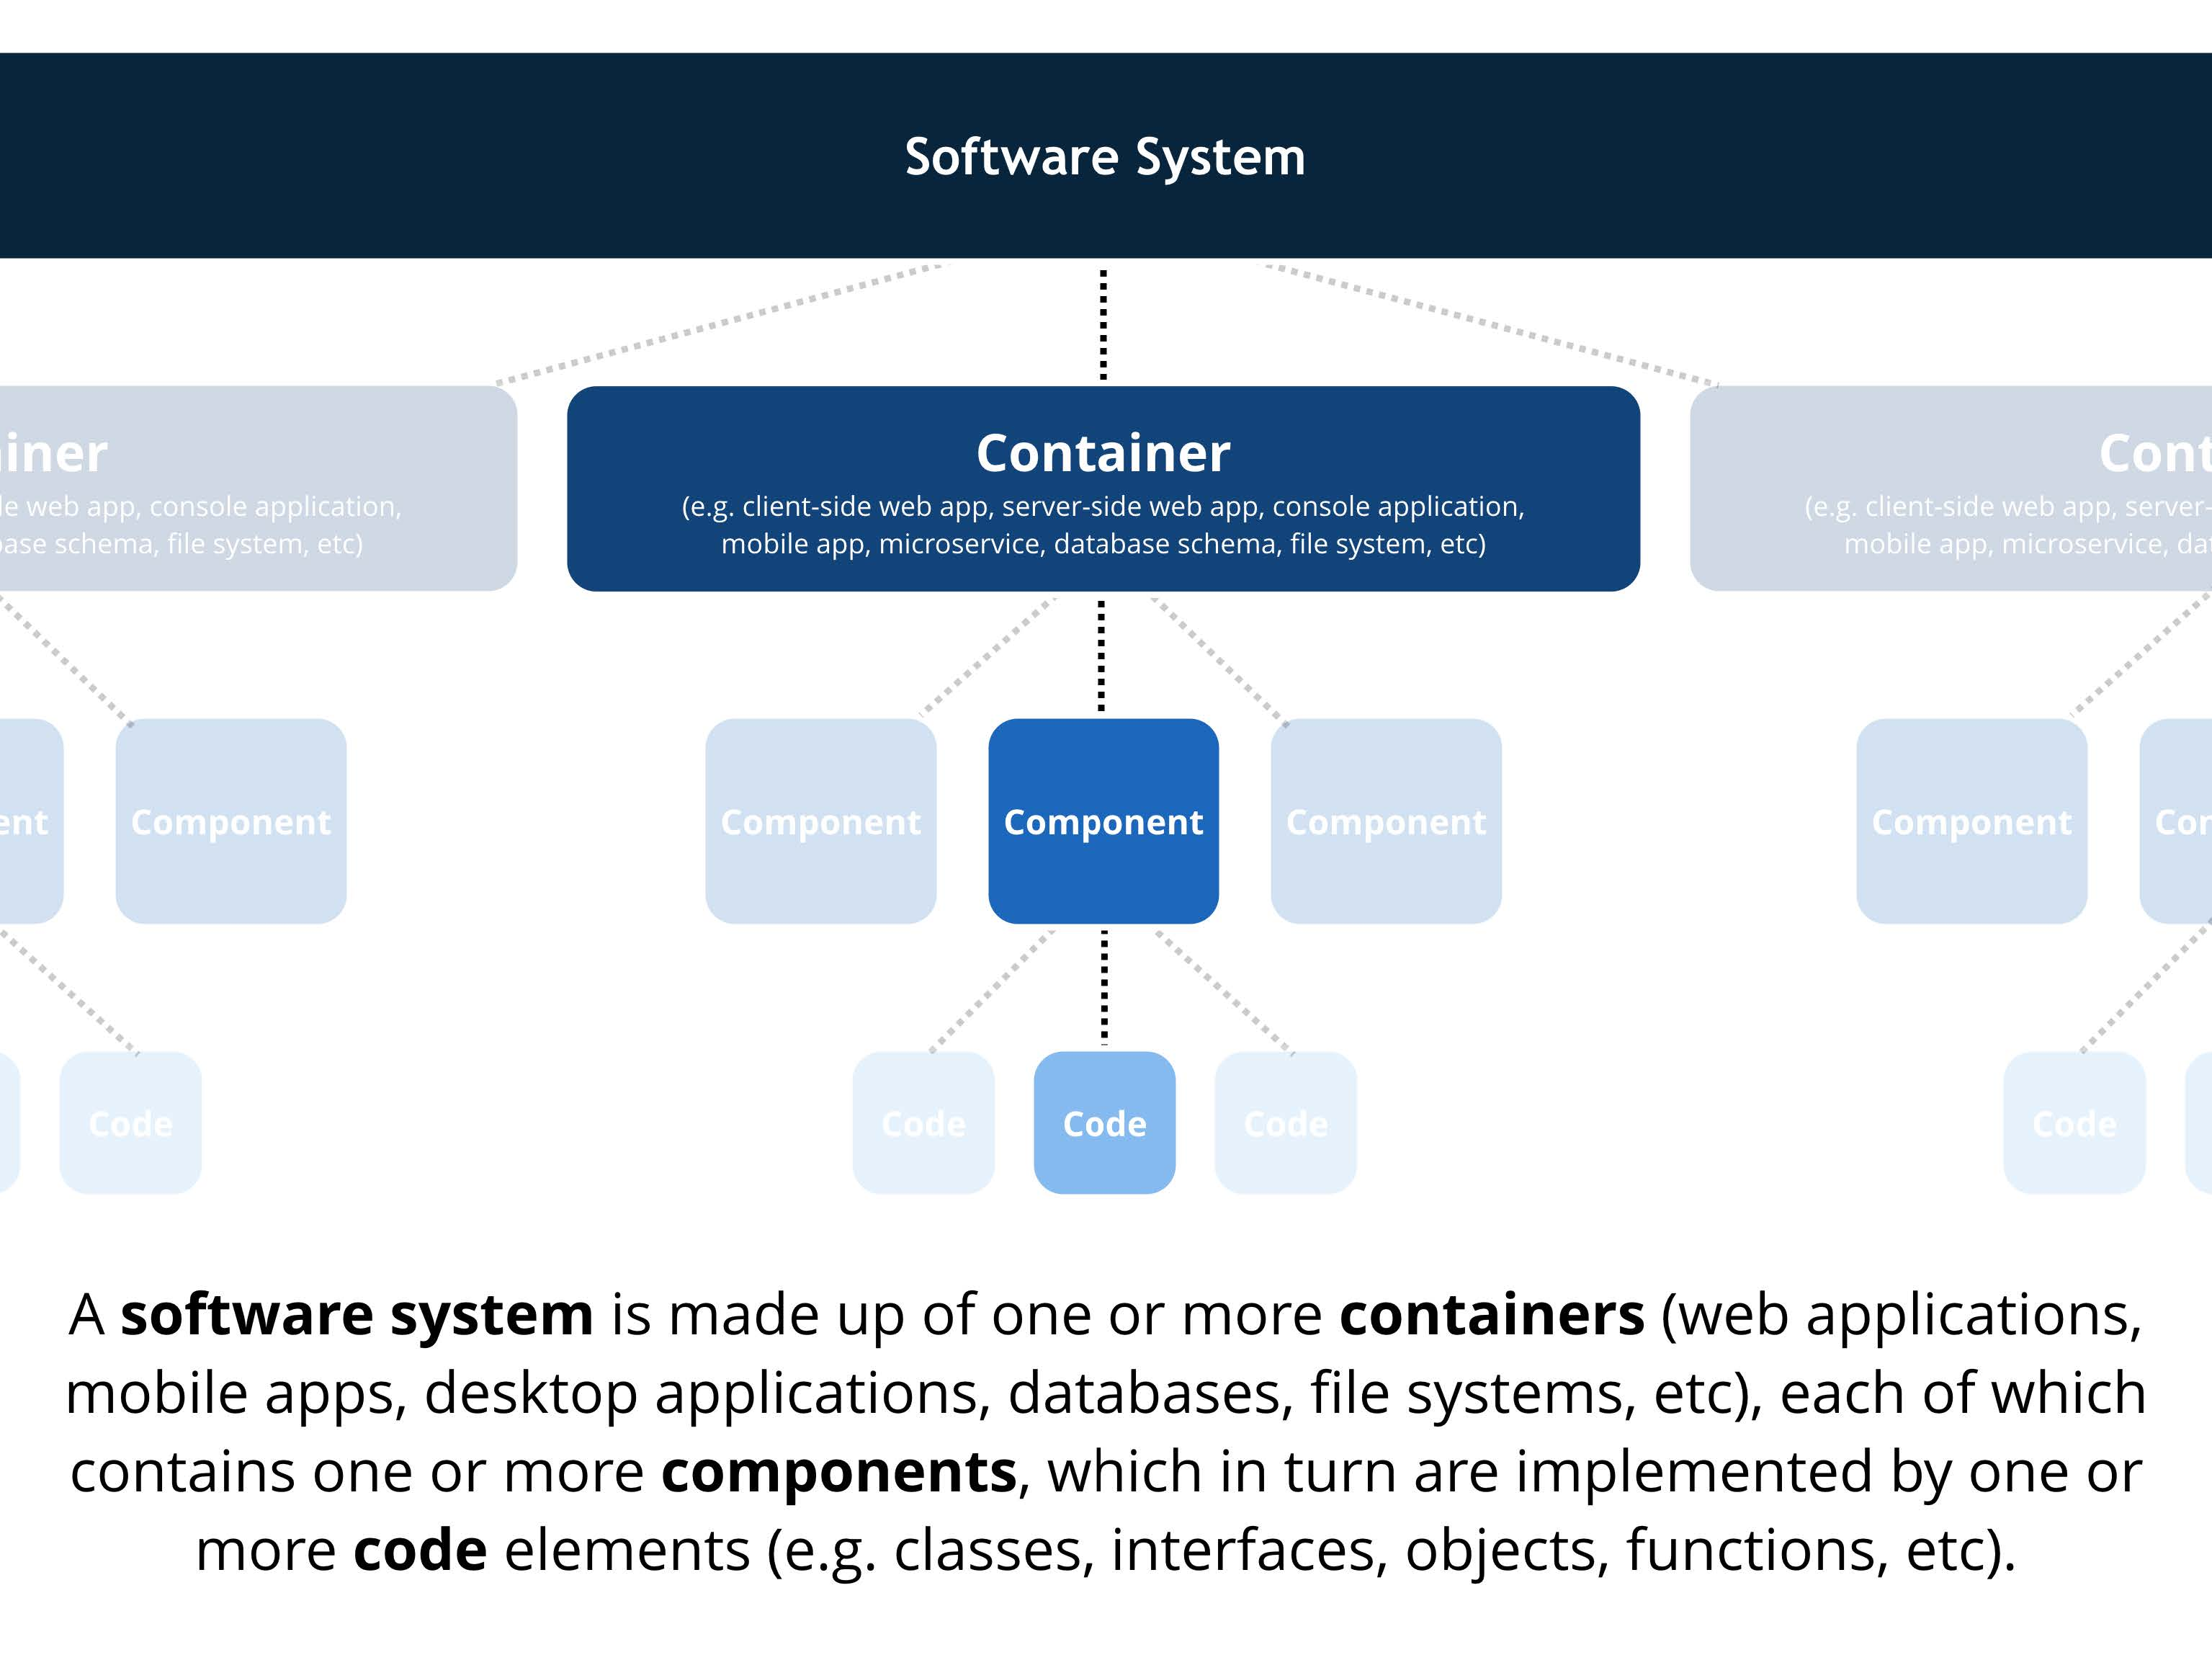
\includegraphics[trim=0 8 0 5,clip,width=0.8\textwidth]{images/c4_terminology.jpg}
    \caption{Levels within the C4 model (figure 2.1 from \cite{brown2022c4}).}
    \label{fig:c4terms}
\end{figure}

\noindent
This leads to describing the static structure of software architecture through four levels of abstraction.
Each level providing detail about parts of the previous level.
\begin{description}
    \item[Context] How the software system fits into the broader context around it.
    \item[Containers] How the containers are connected to deliver system functionality.
    \item[Components] How the components are structured to implement a container's behaviour.
    \item[Code] How the code is structured to implement a component.
\end{description}

\subsection{System Context}
The system context provides the `big picture' perspective of the software system.
It describes the key purpose of the system, who uses it, and with which other systems it interacts.
The context diagram is usually a simple block diagram.
The software system being designed typically sits in the centre of the diagram surrounded by uers and other systems.
The intent is to set the context for thinking about the software system's architecture.
It can also be used to communicate basic structural ideas to non-technical stakeholders.
Figure \ref{fig:c4_context} is a context diagram for the Sahara eCommerce example from section \ref{sec:storeExample}.

\begin{figure}[h]
    \centering
    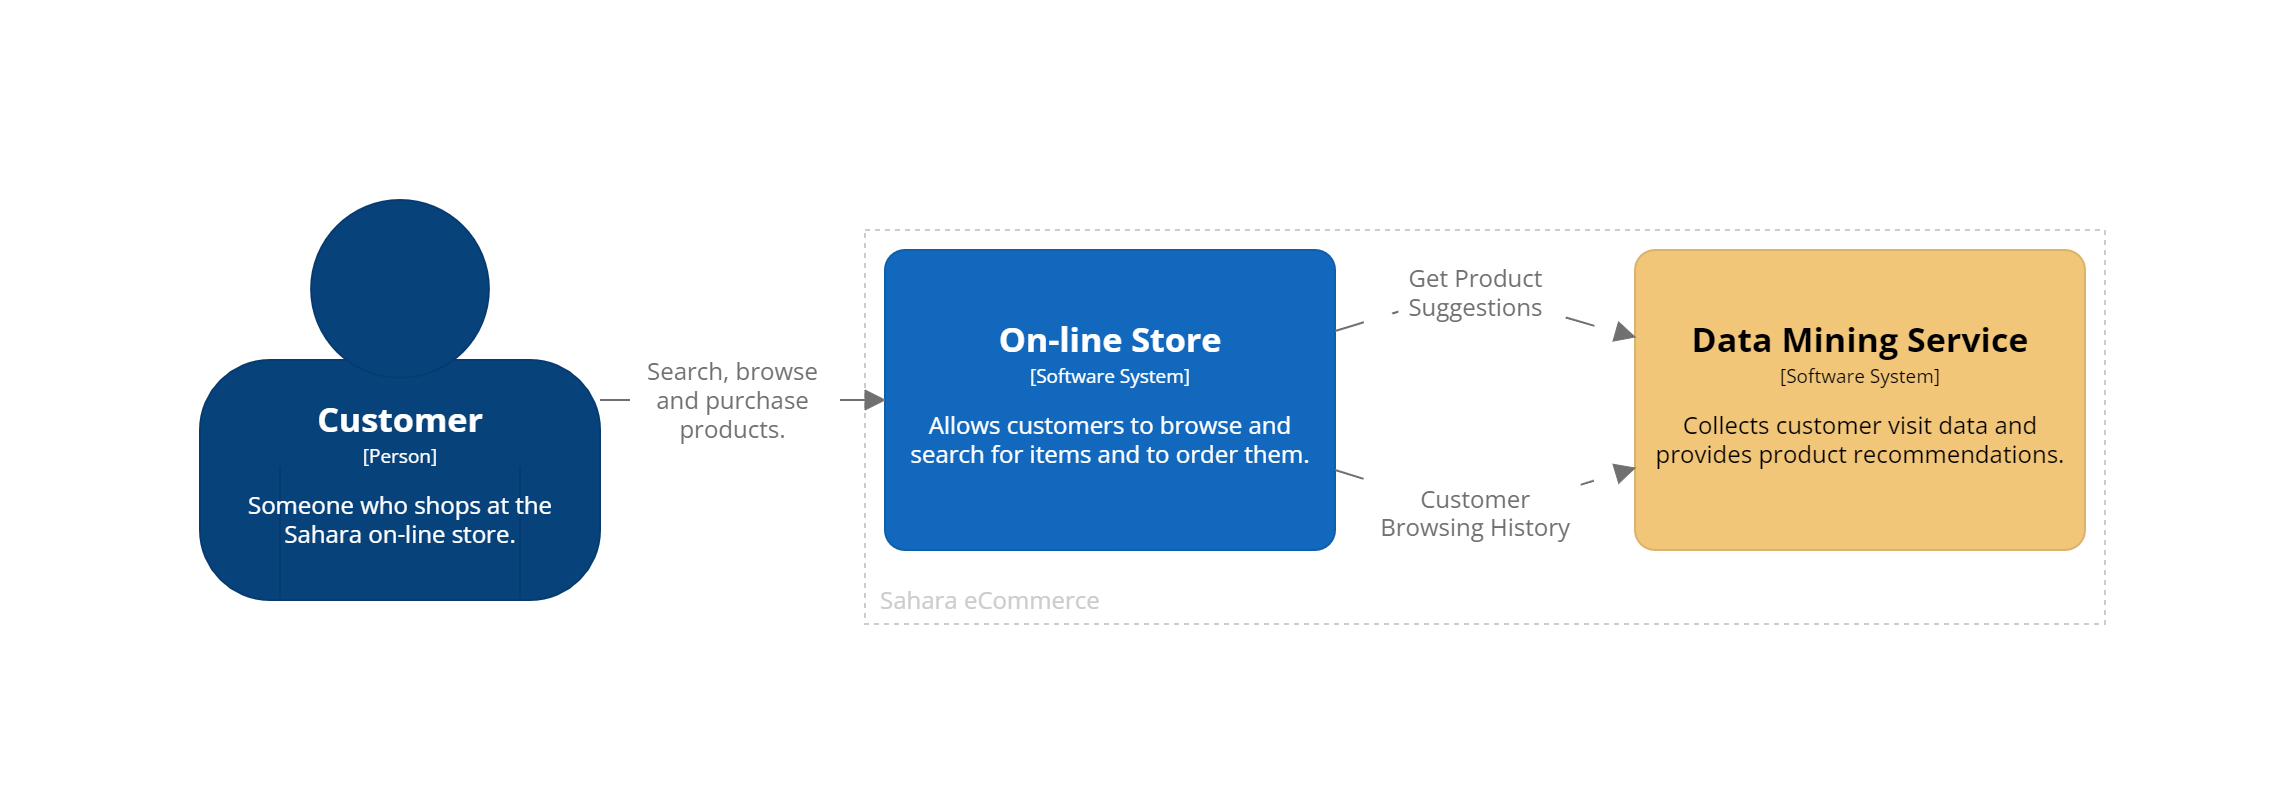
\includegraphics[trim=195 195 198 195,clip,width=\textwidth]{images/c4/context_diagram.png}
    \caption{Context diagram for the Saraha eCommerce on-line store.}
    \label{fig:c4_context}
\end{figure}

\noindent
Figure \ref{fig:c4_context_key} is the key to help interpret the context diagram.
A key is important for C4 diagrams, as they do not have a formal syntax and specification like UML diagrams.

\begin{figure}[h!]
    \centering
    \begin{adjustwidth}{-7.5mm}{-7.5mm}
        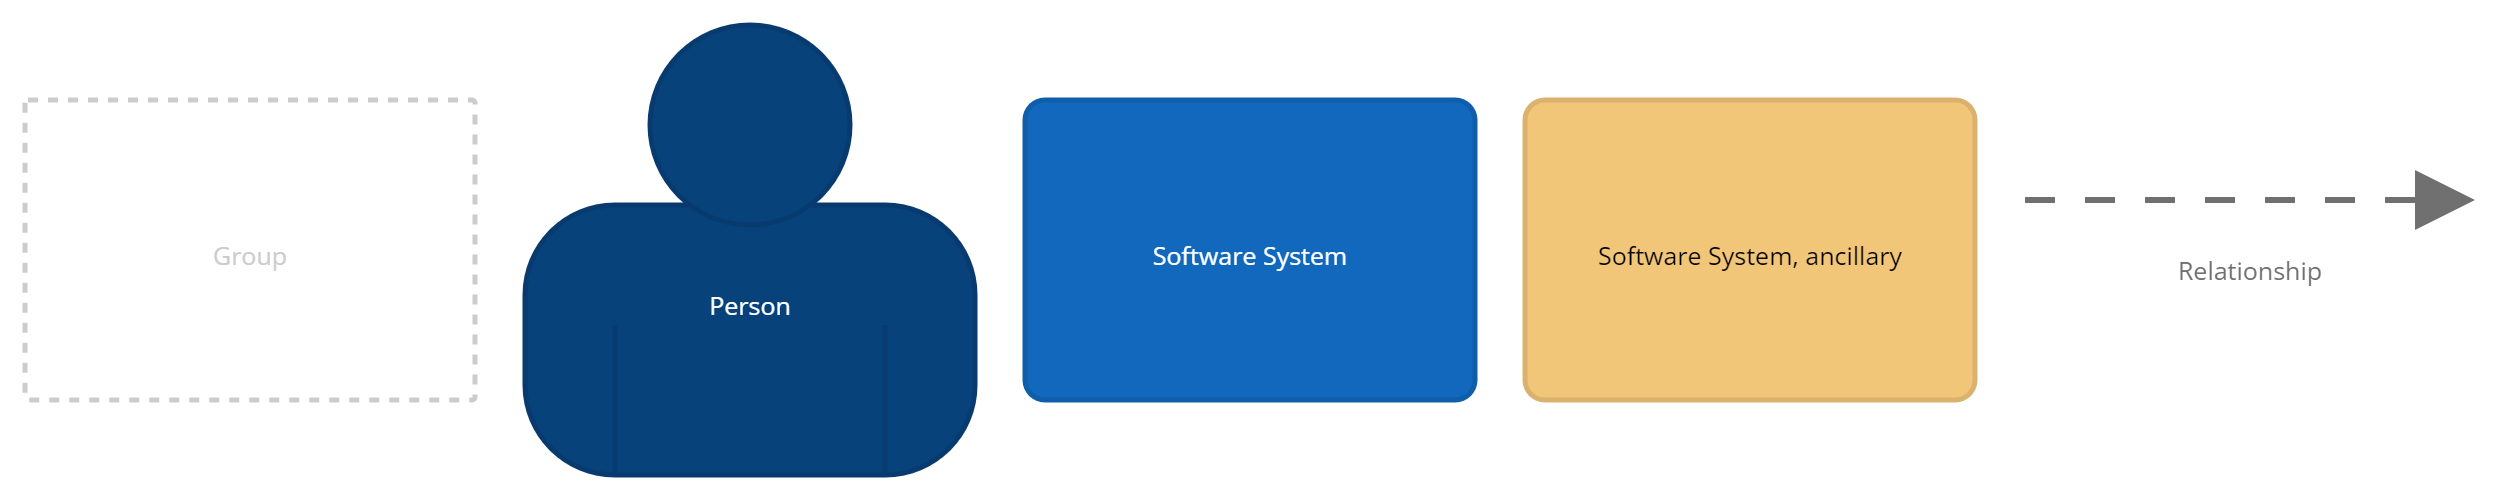
\includegraphics[trim=20 15 20 18,clip,width=0.95\paperwidth]{images/c4/context_diagram-key.png}
    \end{adjustwidth}
    \caption{Context diagram key.}
    \label{fig:c4_context_key}
\end{figure}

\noindent
The context diagram situates the on-line store software system in the environment in which it will be used.
There are customers who shop at the on-line store, which is part of Sahara eCommerce's software ecosystem.
The on-line store uses a data mining service that is also implemented by the company.
The two key relationships between the on-line store and the data mining service are 
that the on-line store sends customer browsing data to the service,
and that the on-line store requests the data mining service to recommend products for a customer.

In C4, arrows are used to indicate the main direction of the relationship, not the flow of data.
So, in this example, the arrow points from the on-line store to the data mining service as it is the store that manages the communication.

In UML, a high-level use case diagram can be used to convey similar information to the C4 context diagram.
Kruchten's ``4+1 View Model of Software Architecture'' \cite{4+1-model} uses this approach.

\subsection{Containers}
Container diagrams provide an overview of the software architecture.
They describe the main structure of the software system and the technologies selected to implement these aspects of the system.
Containers are `blocks' of code that can be independently deployed and executed.
Examples of containers are web or mobile applications, databases, message buses, ....
It is important to note that this is not a type of deployment diagram.
Containers may be deployed on the same computing infrastructure or on different devices.
While the container diagram does not explicitly show computing infrastructure, some of the infrastructure may be implied by the types of containers.
Decisions about how containers are connected and communicate have major implications for how the components and code will be designed and deployed.
Figure~\ref{fig:c4_container_store} is a container diagram for the on-line store.

\begin{figure}[h!]
    \centering
    \begin{adjustwidth}{-9mm}{-9mm}
        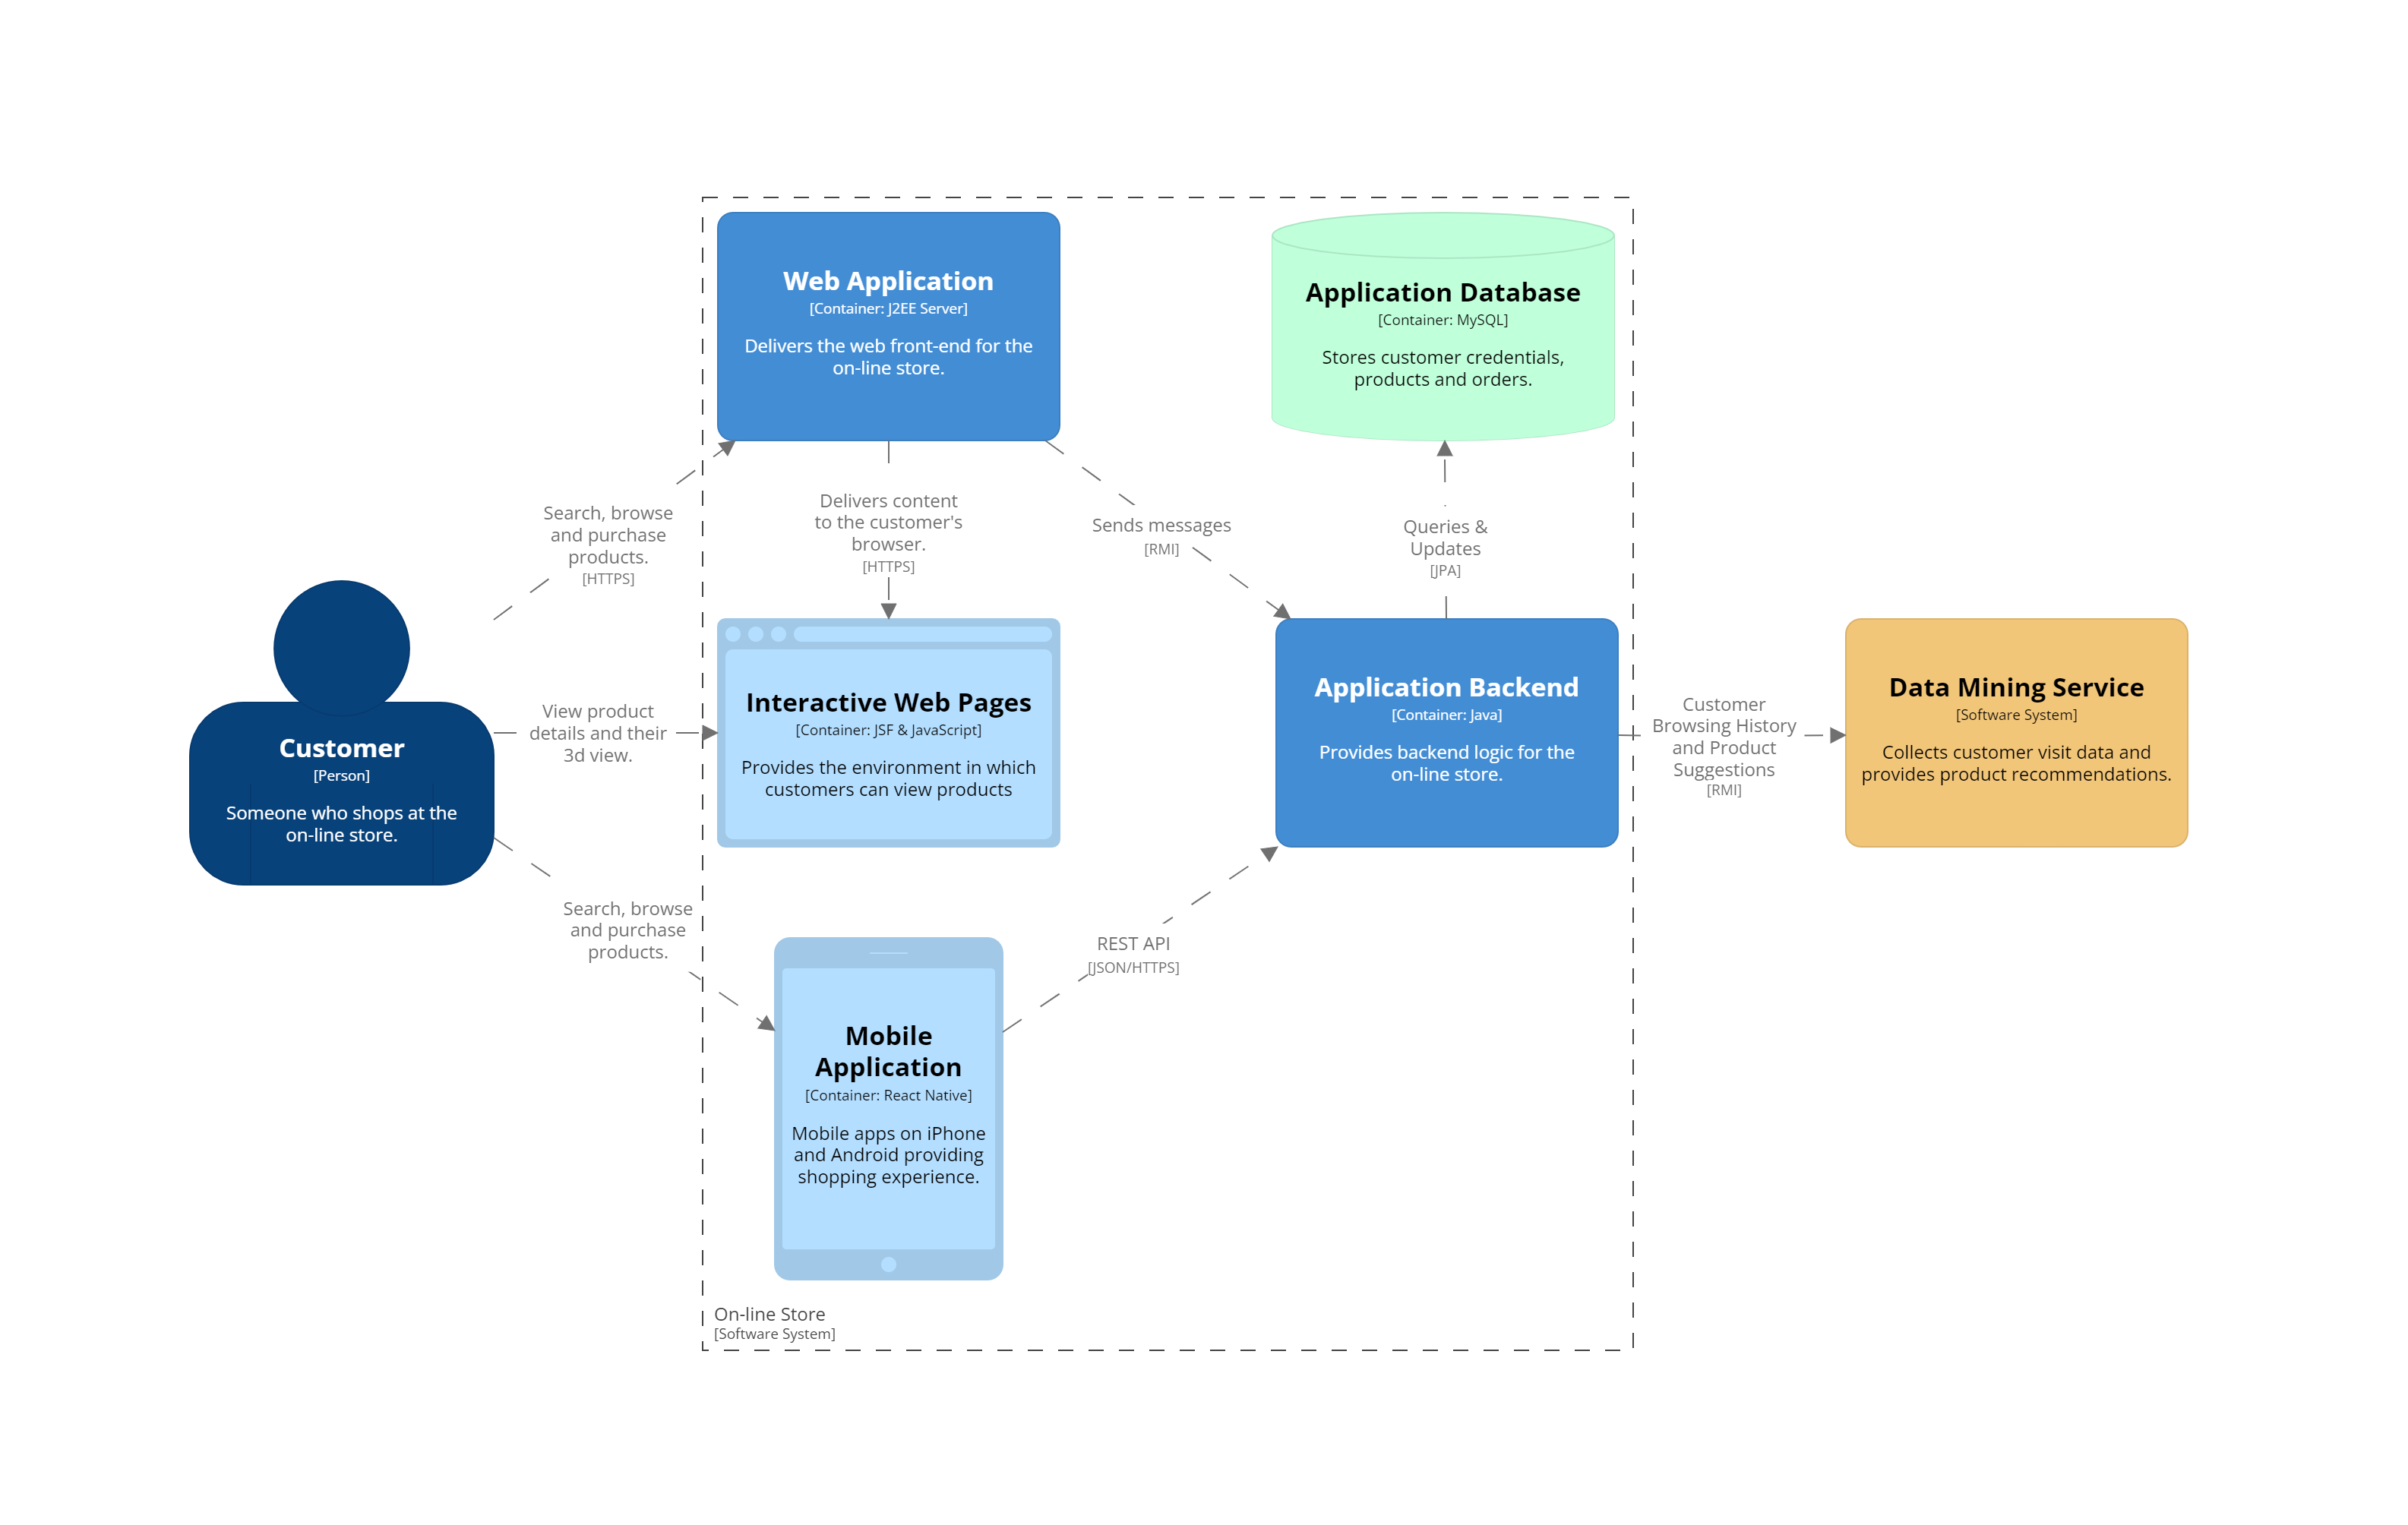
\includegraphics[trim=250 226 286 258,clip,width=0.96\paperwidth]{images/c4/store_container_diagram.png}
    \end{adjustwidth}
    \caption{Container diagram for the on-line store software system.}
    \label{fig:c4_container_store}
\end{figure}

\noindent
Customers can access the on-line store through either web or mobile applications.
The \texttt{Interactive Web Pages} container indicates that some of the web application's behaviour is delivered in a separate container.
This indicates similar information as in figure \ref{fig:deploymentDiagram},
where the customer's computer and browser were included in the deployment diagram to show that a JavaScript component was to be deployed to run in the browser.

The web and mobile applications both communicate with the application backend, via different protocols, to provide the logical behaviour of the on-line store.
The backend uses JPA to perform database operations on the application's database.

To provide a link to the context diagram, a container diagram usually shows which containers communicate with which external elements.
The text inside the square brackets in a container, and on a relationship, indicates the technology used to implement that container or relationship.

\begin{figure}[h!]
    \centering
    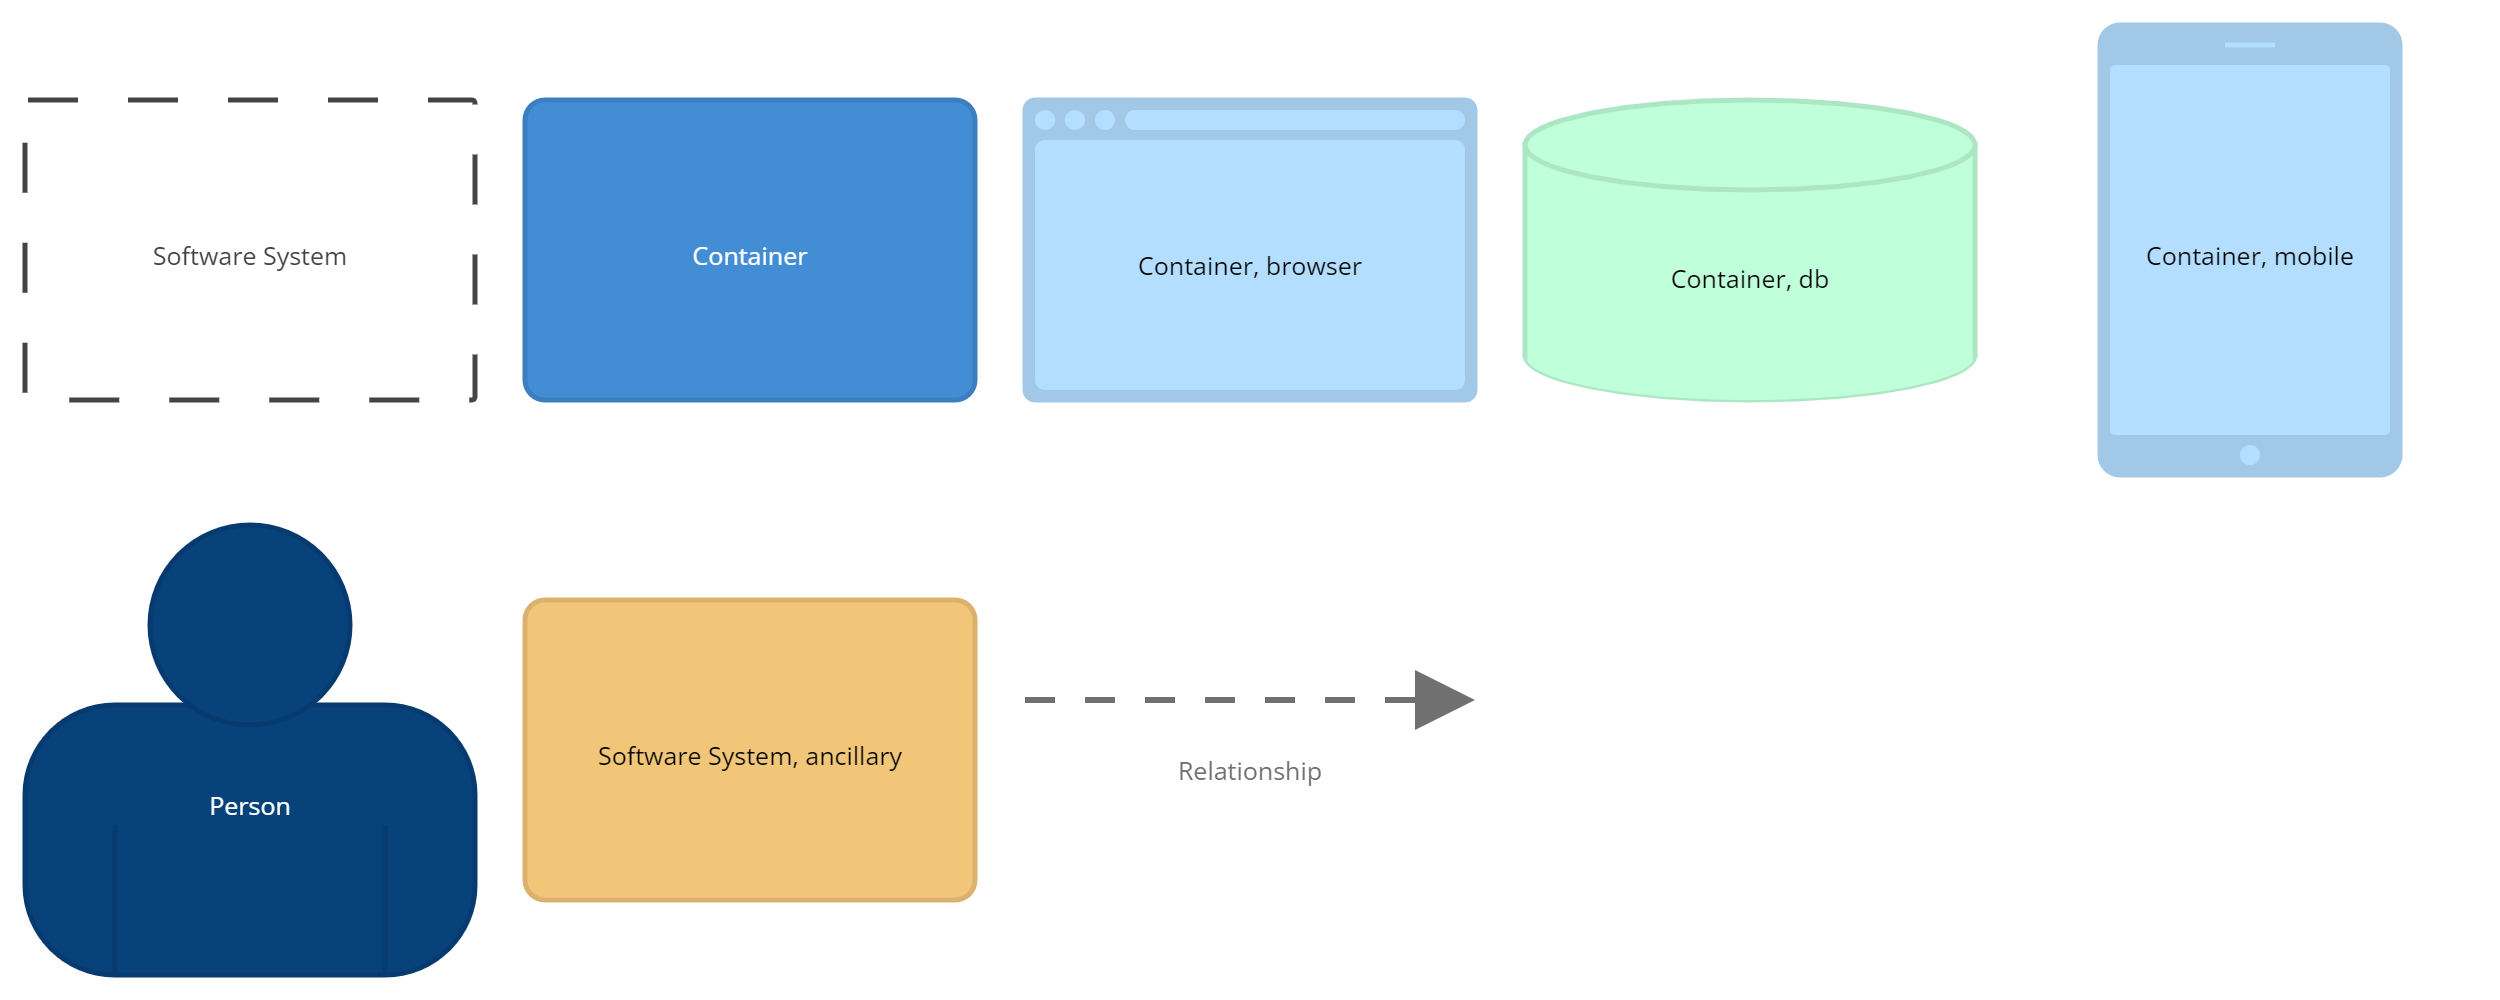
\includegraphics[trim=24 21 98 26,clip,width=\textwidth]{images/c4/container_diagram-key.png}
    \caption{Container diagram key.}
    \label{fig:c4_container_key}
\end{figure}

While a container diagram does not explicitly show computing infrastructure,
some of it can be implied by the types of containers in the diagram.
Clearly, the mobile app and the code running in the interactive web pages
have to be separate computing platforms to the rest of the on-line store's software system.

Colours and icons can be used to provide further information in the diagrams.
The diagram key in figure~\ref{fig:c4_container_key} explains the purpose of each icon and colour.
UML also allows you to use icons and colours to add further information to a model, it is just difficult to do in many UML modelling tools.

\filbreak
\noindent
The data mining service software system (figure \ref{fig:c4_container_datamining}) has three main containers.

\texttt{Data Mining Interface} provides the interface used to interact with the data mining service.
It accepts data to store for future data mining.
It returns suggestions based on requests from external systems, such as the on-line store.

\texttt{Data Mining Process} performs the data mining logic.

\texttt{Data Warehouse} stores the data and provides an SQL-based query system to manipulate the data.

\begin{center}
    \begin{adjustwidth}{-5mm}{-5mm}
        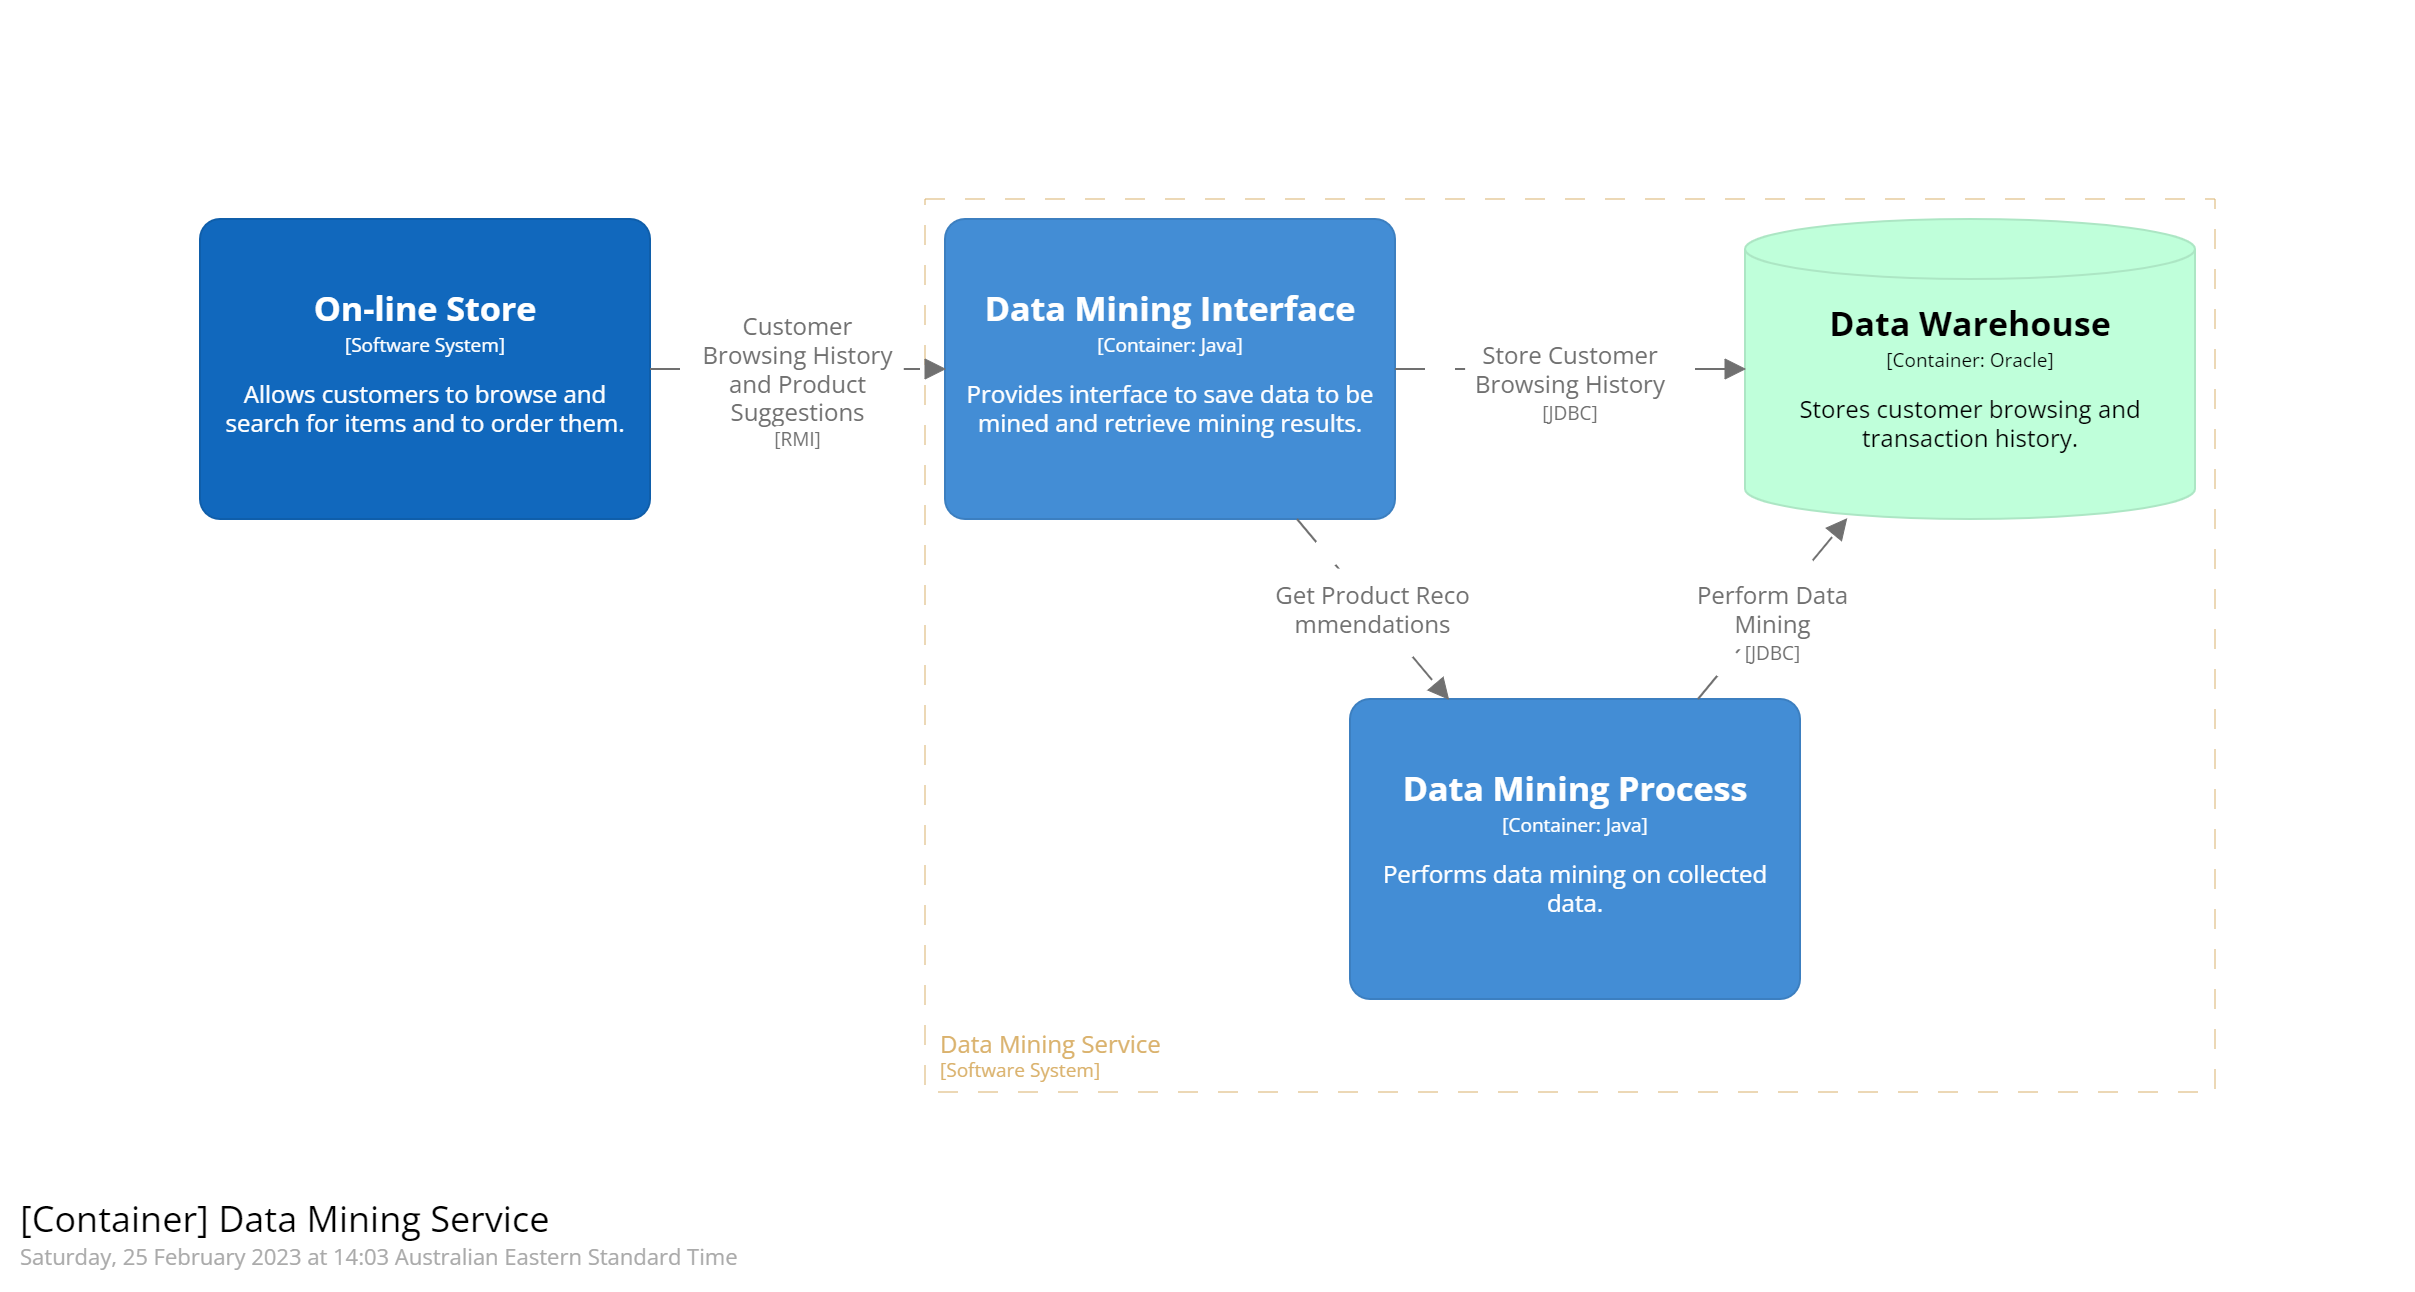
\includegraphics[trim=185 185 185 185,clip,width=0.92\paperwidth]{images/c4/datamining_container_diagram.png}
    \end{adjustwidth}
    \captionof{figure}{Container diagram for the data mining service software system.}
    \label{fig:c4_container_datamining}
\end{center}

\subsection{Components}
Component diagrams describe the major parts of containers and how they are connected.
Components should describe their important responsibilities and the technology used to implement them
(e.g. using React to implement a web frontend component).
Like a container diagram, a component diagram can include elements from higher level diagrams
to provide context of how the components interact with elements outside of the container.

\begin{figure}[h!]
    \centering
    \begin{adjustwidth}{-8.5mm}{-8.5mm}
        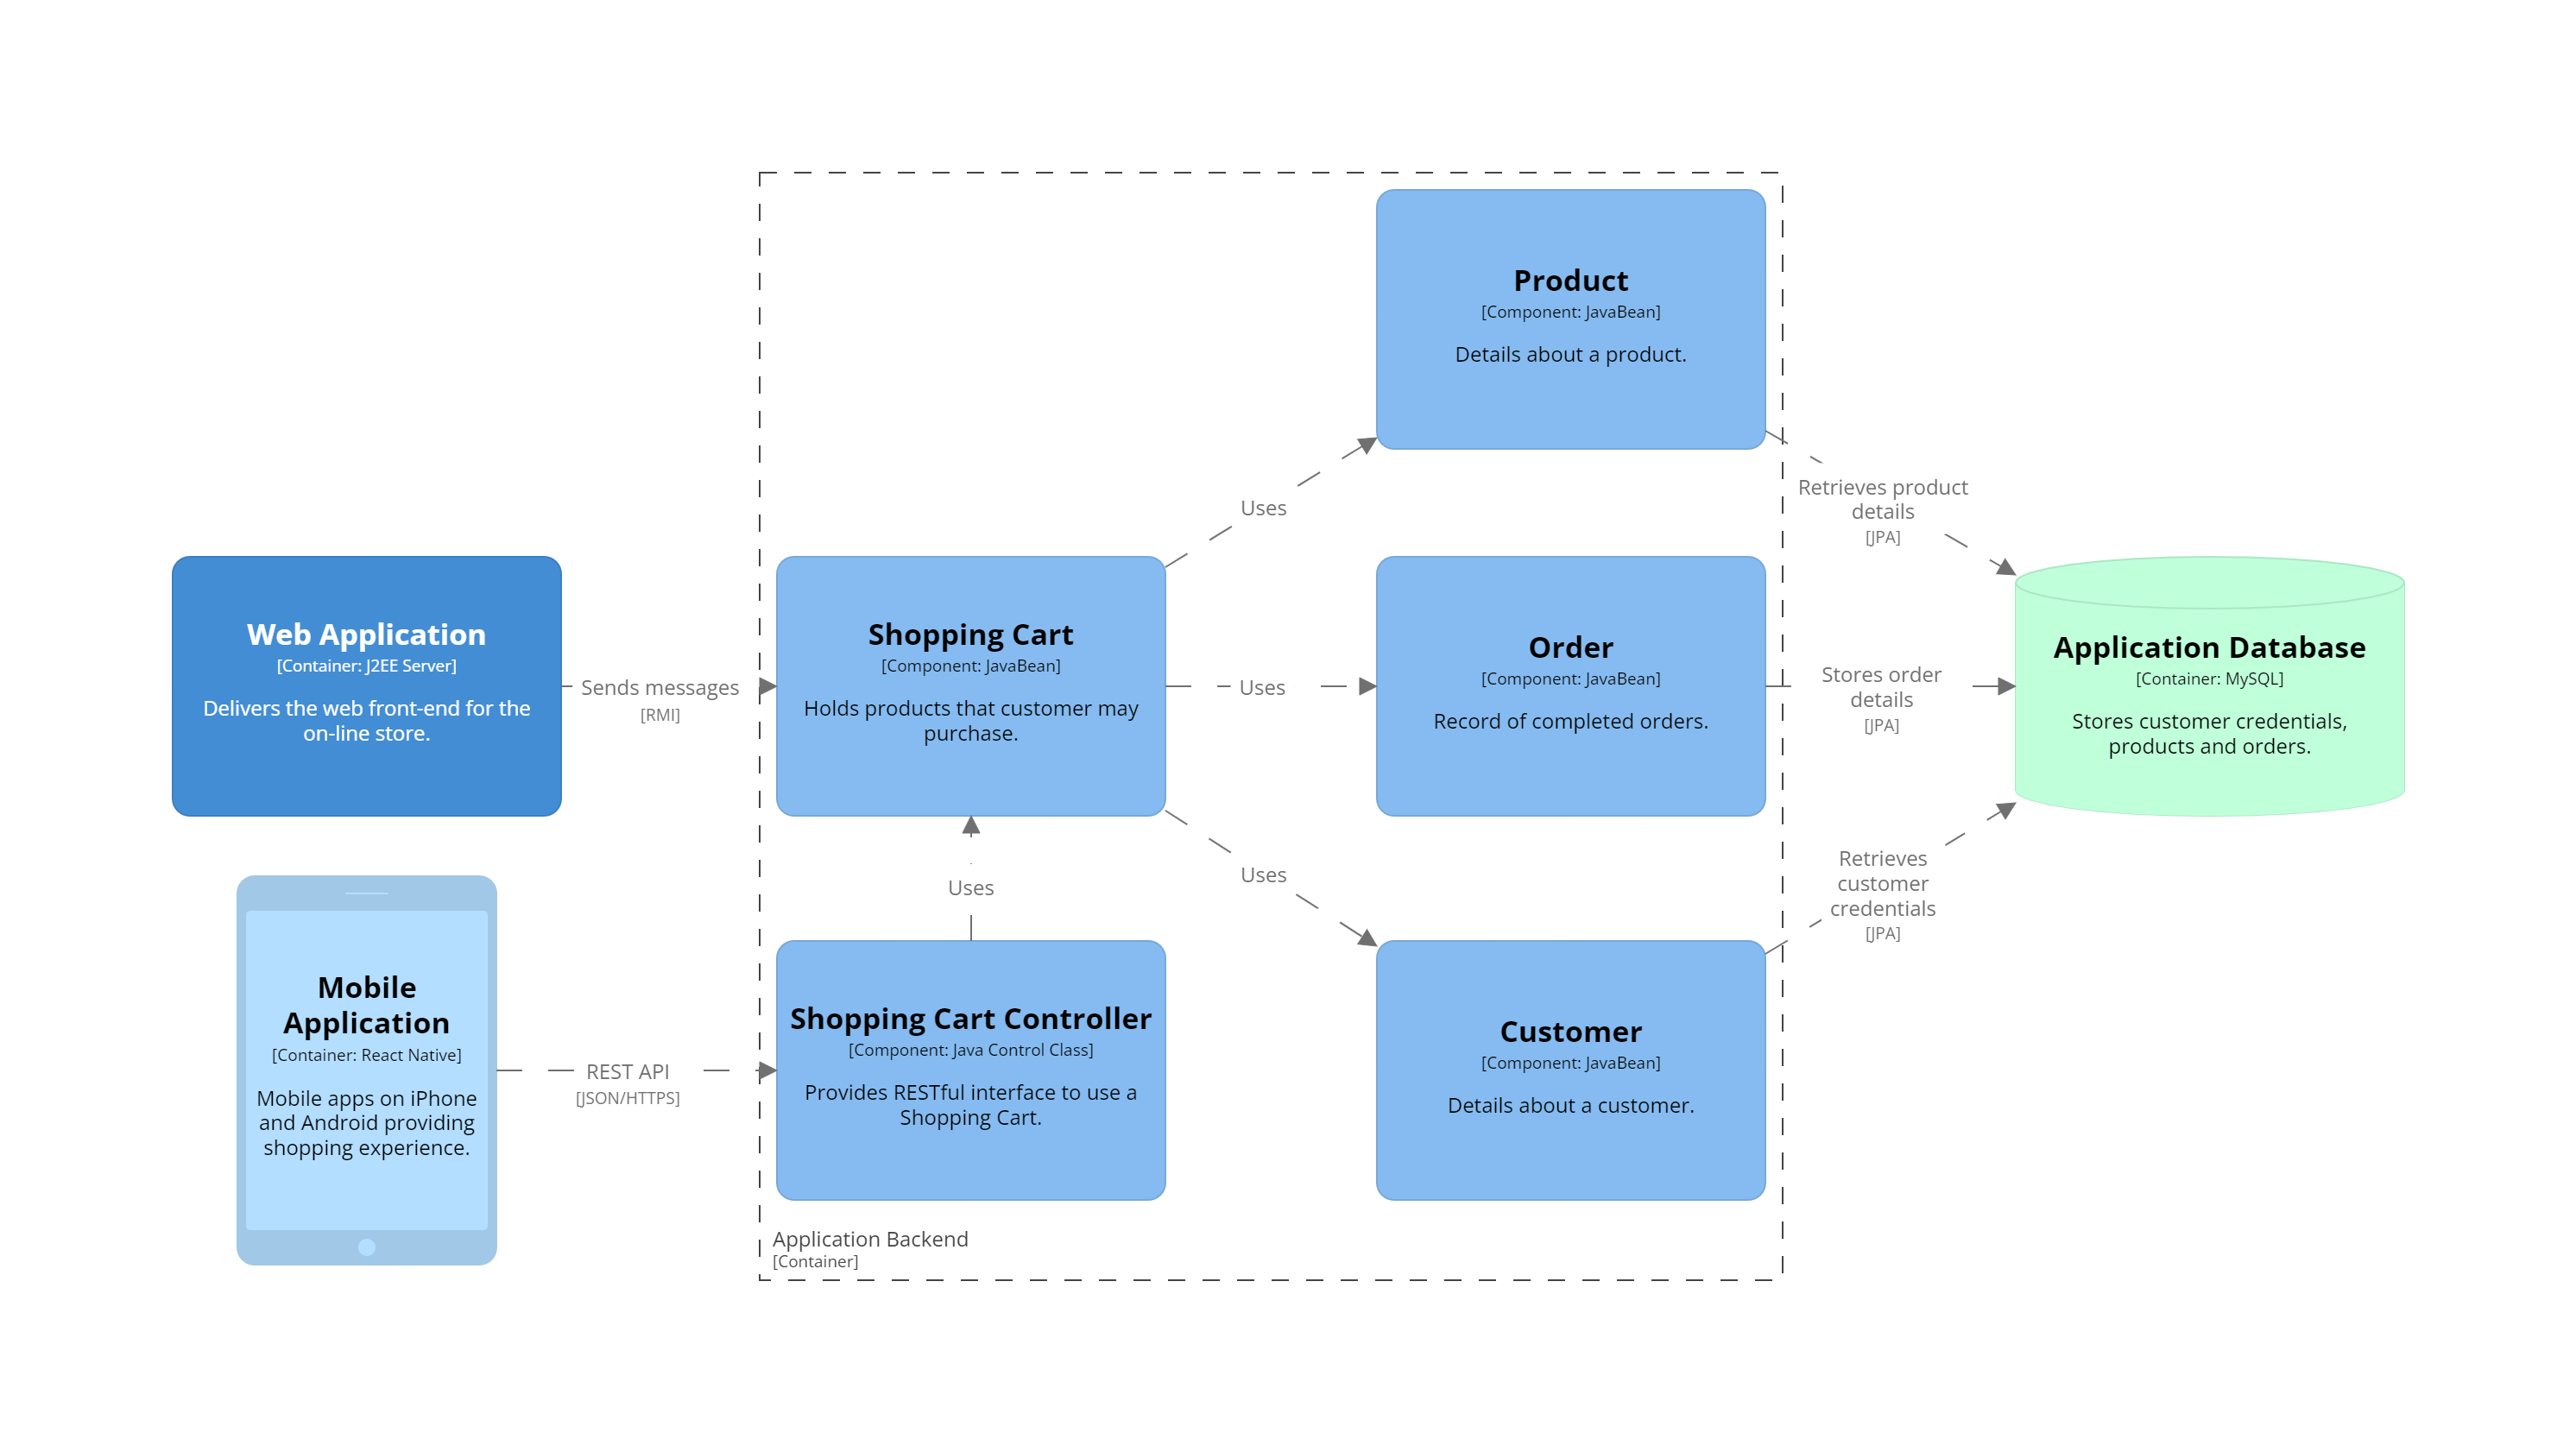
\includegraphics[trim=190 185 197 198,clip,width=0.96\paperwidth]{images/c4/appbackend_component_diagram.png}
    \end{adjustwidth}
    \caption{Component diagram for the application backend container.}
    \label{fig:c4_component_appbackend}
\end{figure}

\noindent
In figure \ref{fig:c4_component_appbackend}, the application backend is divided into five main components.
The \texttt{Shopping Cart} component provides the backend logic of implementing a shopping cart.
The web application interacts with the \texttt{Shopping Cart} component via RMI.
The \texttt{Shopping Cart} component would provide interfaces for this interaction.
The mobile applications use a REST API provided by the \texttt{Shopping Cart Controller} component to interact with the \texttt{Shopping Cart}.
\texttt{Shopping Cart} uses the \texttt{Product}, \texttt{Order} and \texttt{Customer} components to deliver its behaviour.
These are all implemented as Java beans.

The \texttt{Product}, \texttt{Order} and \texttt{Customer} components use JPA to retrieve and store data in the application database.
(As indicated in section \ref{sec:CnC_view}, only the components related to managing the shopping cart are shown in this example.)

Figure \ref{fig:c4_component_key}, shows the icons and colours used to represent different elements in the component diagrams.

\begin{figure}[h!]
    \centering
    \begin{adjustwidth}{-7.5mm}{-7.5mm}
        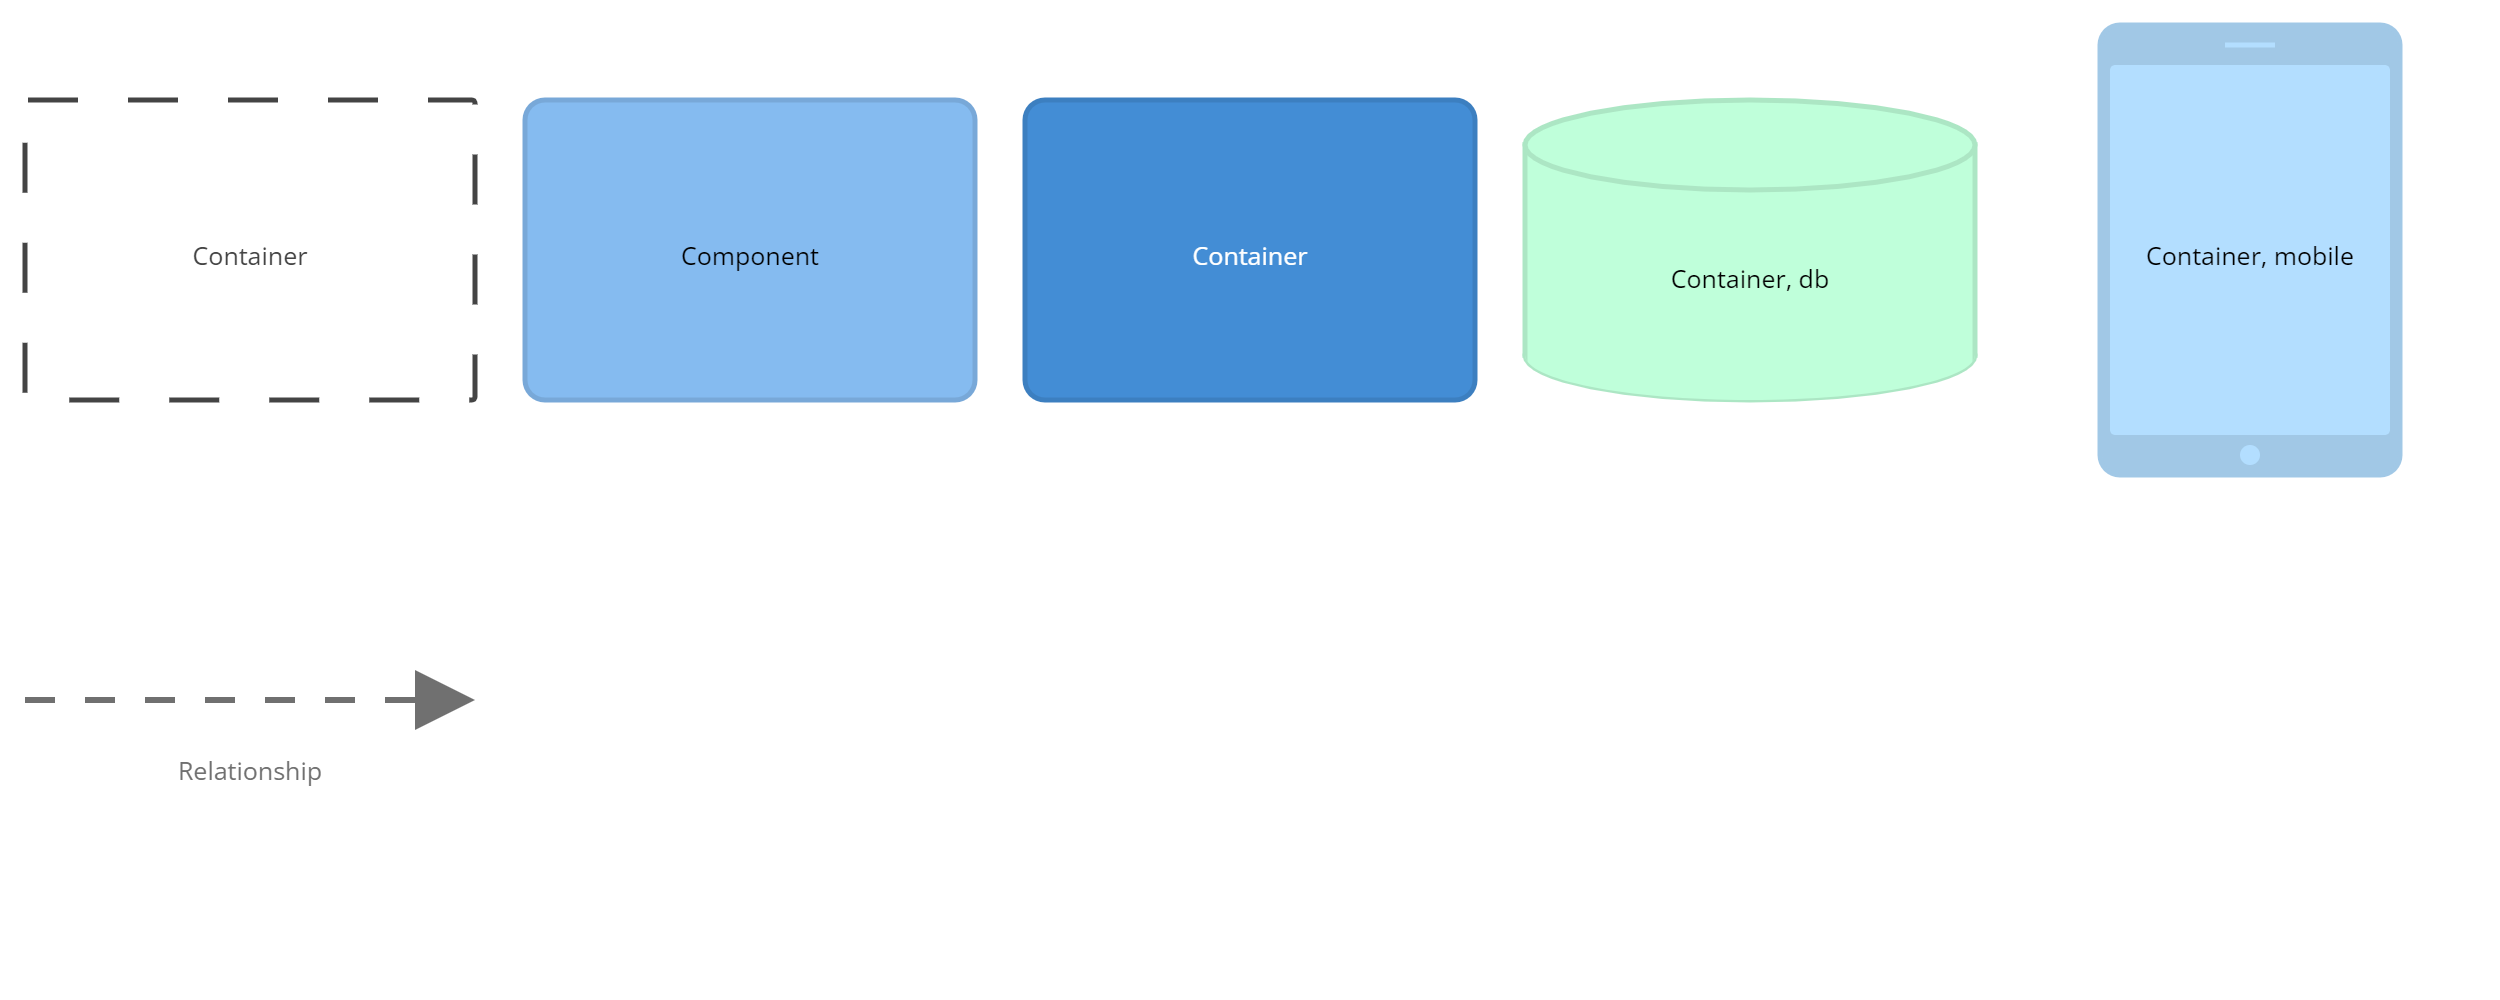
\includegraphics[trim=15 210 90 20,clip,width=0.95\paperwidth]{images/c4/component_diagram-key.png}
    \end{adjustwidth}
    \caption{Component diagram key.}
    \label{fig:c4_component_key}
\end{figure}

\newpage
\noindent
Figure \ref{fig:c4_component_webapp} shows the components that provide the frontend behaviour
of browsing for products, adding them to the shopping cart, and purchasing them.

\begin{figure}[h!]
    \centering
    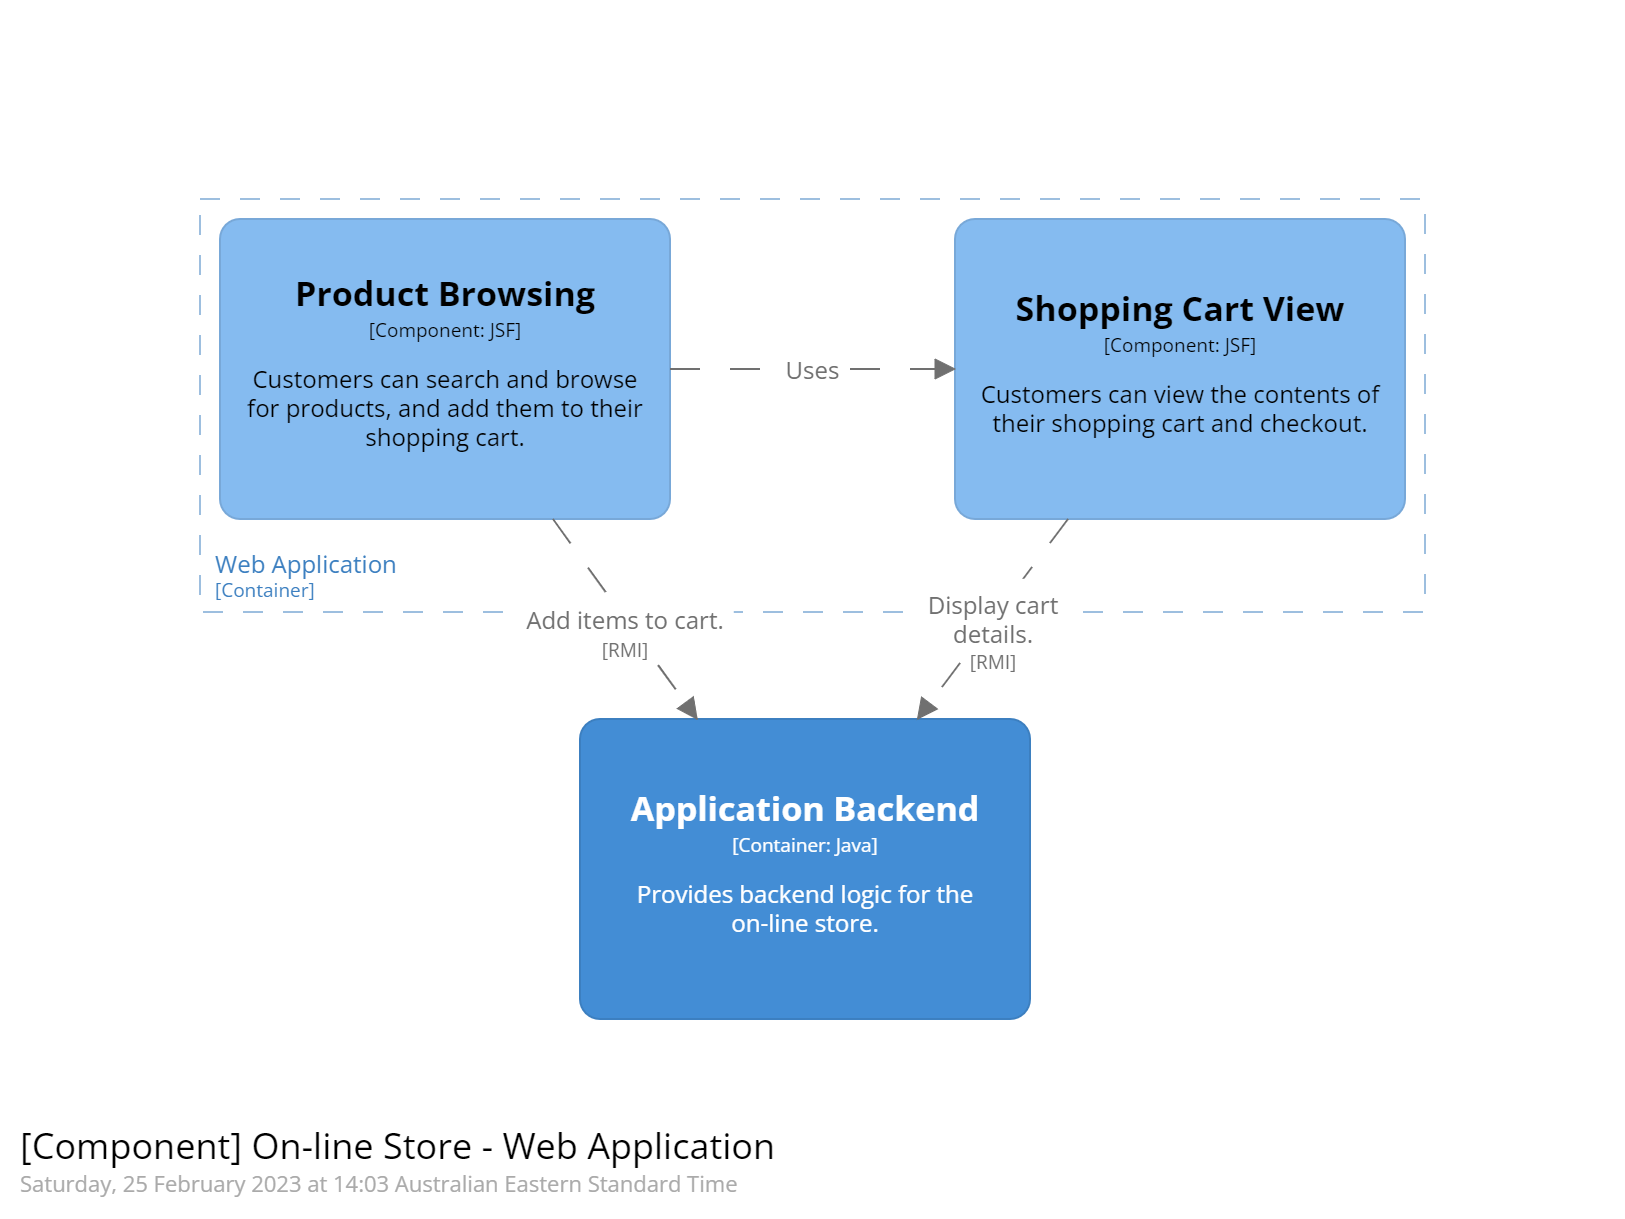
\includegraphics[trim=190 193 190 195,clip,width=0.65\textwidth]{images/c4/webapp_component_diagram.png}
    \caption{Component diagram for the web application container.}
    \label{fig:c4_component_webapp}
\end{figure}

\noindent
Figure \ref{fig:c4_component_browser}, shows that the \texttt{Product Animator} component
is downloaded from the web application to the customer's browser and that it is implemented in JavaScript.
This provides similar information about the \texttt{Product Animator} component, as described in section \ref{sec:storeAllocView}.

\begin{figure}[h!]
    \centering
    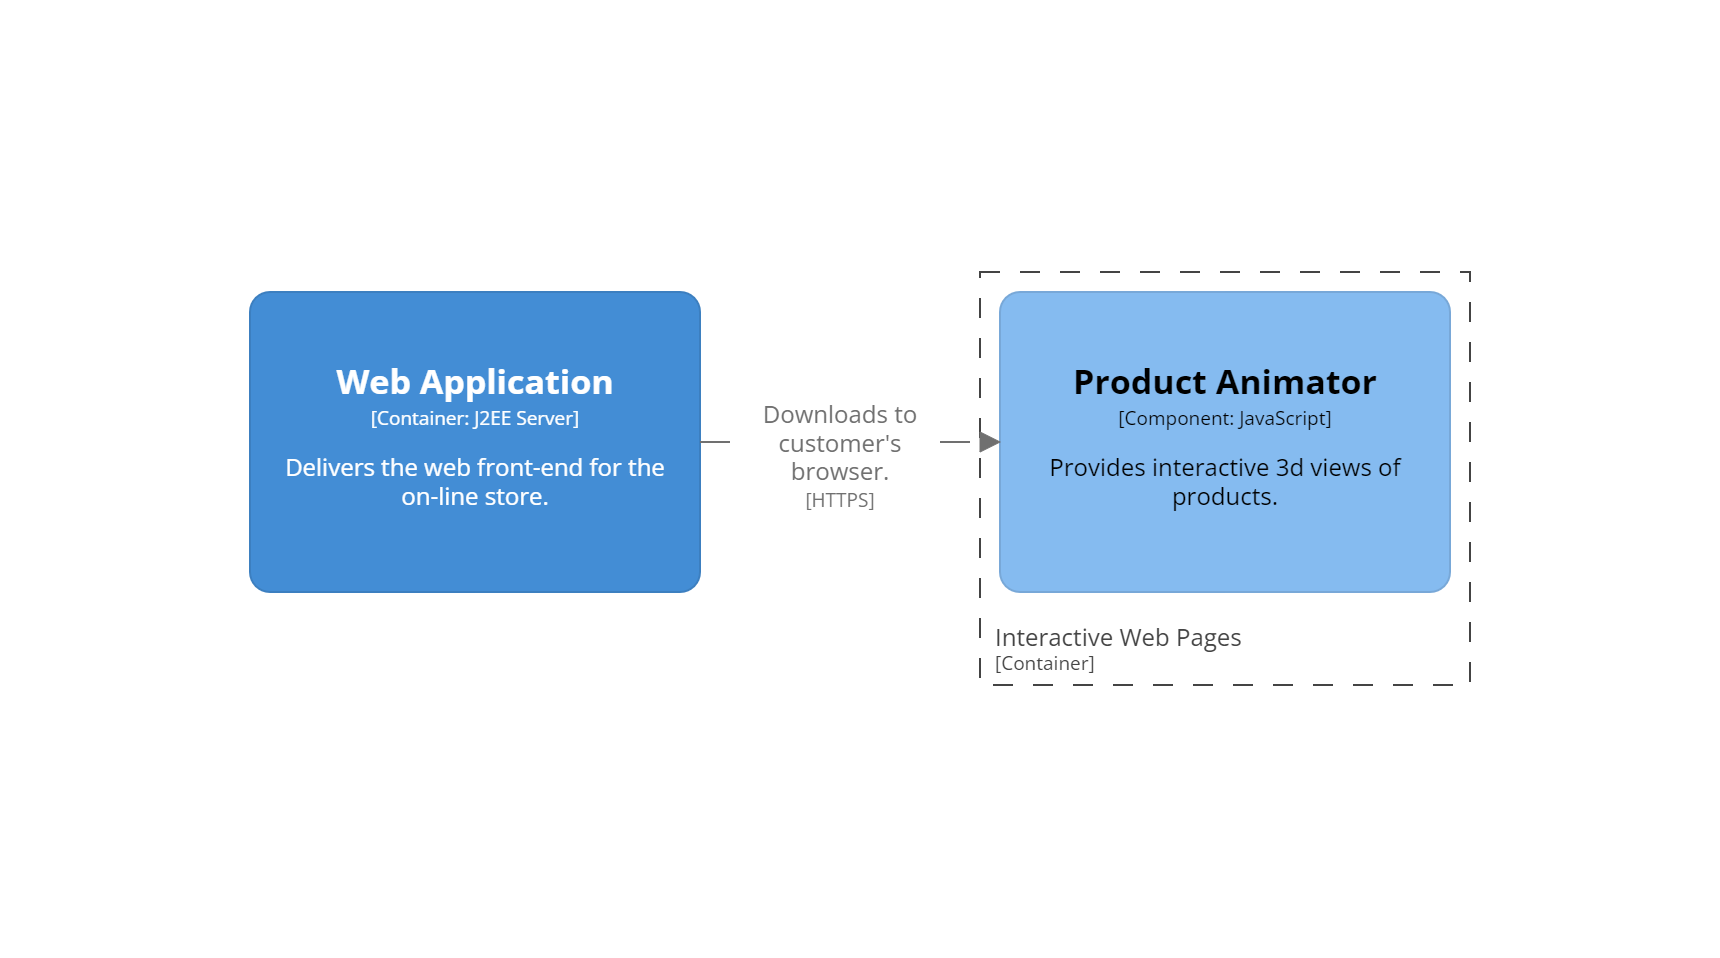
\includegraphics[trim=245 265 245 270,clip,width=0.65\textwidth]{images/c4/browser_component_diagram.png}
    \caption{Component diagram for the interactive web pages container.}
    \label{fig:c4_component_browser}
\end{figure}

\subsubsection{Component Diagram Detail}
There may be some components that are important parts of the software design,
but which may not necessarily be included in component diagrams.
For example, a logging component is an important part of many software systems.
But, due to the nature of a logging component, most other components will use it.
Adding it to component diagrams will often clutter the diagrams without adding much useful information.
Usually it is better to add a note indicating which logging component is used in the system.
If it is helpful to indicate which components use the logging component,
it may be better to colour code these components or use an icon to represent that they use the logging component.

\subsection{Code}
The code-level diagrams describe the structure of the code that implements a component.
The intent is to provide a visual representation of the important aspects of the code's structure.
Rarely do you need to provide all the detail that replicates the source code.
(The source code could be considered a fifth level to the C4 model.)

The C4 model suggests using diagrams appropriate to your programming paradigm.
Assuming the implementation is in an object-oriented language, a UML class diagram would be an appropriate way to model the design of the code.
Figure \ref{fig:classDiagram}, from section \ref{sec_moduleView},
would be an example class diagram of how the \texttt{Shopping Cart} component is implemented.

\subsection{Dynamic}
Dynamic diagrams in C4 are similar to UML communication diagrams.
(Communication and sequence diagrams are types of interaction diagrams.
They show the same information but with different visual emphasis.
Sequence diagrams focus on the time or ordered sequence of events that occur in a scenario.
Communication diagrams focus on the links and extent of communication between objects.)

As was mentioned about behavioural structures in sections \ref{sec:behaviourStruct} and \ref{sec:detailedBehaviourStruct},
dynamic diagrams are usually only provided to explain how the architecture delivers complex behaviour.

Figure \ref{fig:c4_dynamic} provides an overview of how the
\texttt{Product Browsing} component in the \texttt{Web Application} container collaborates with the
\texttt{Shopping Cart} component in the \texttt{Application Backend} container
to deliver the behaviour of a customer adding a product to their shopping cart.
It also shows the communication between the \texttt{Shopping Cart} component and the application database.

\begin{figure}[h!]
    \centering
    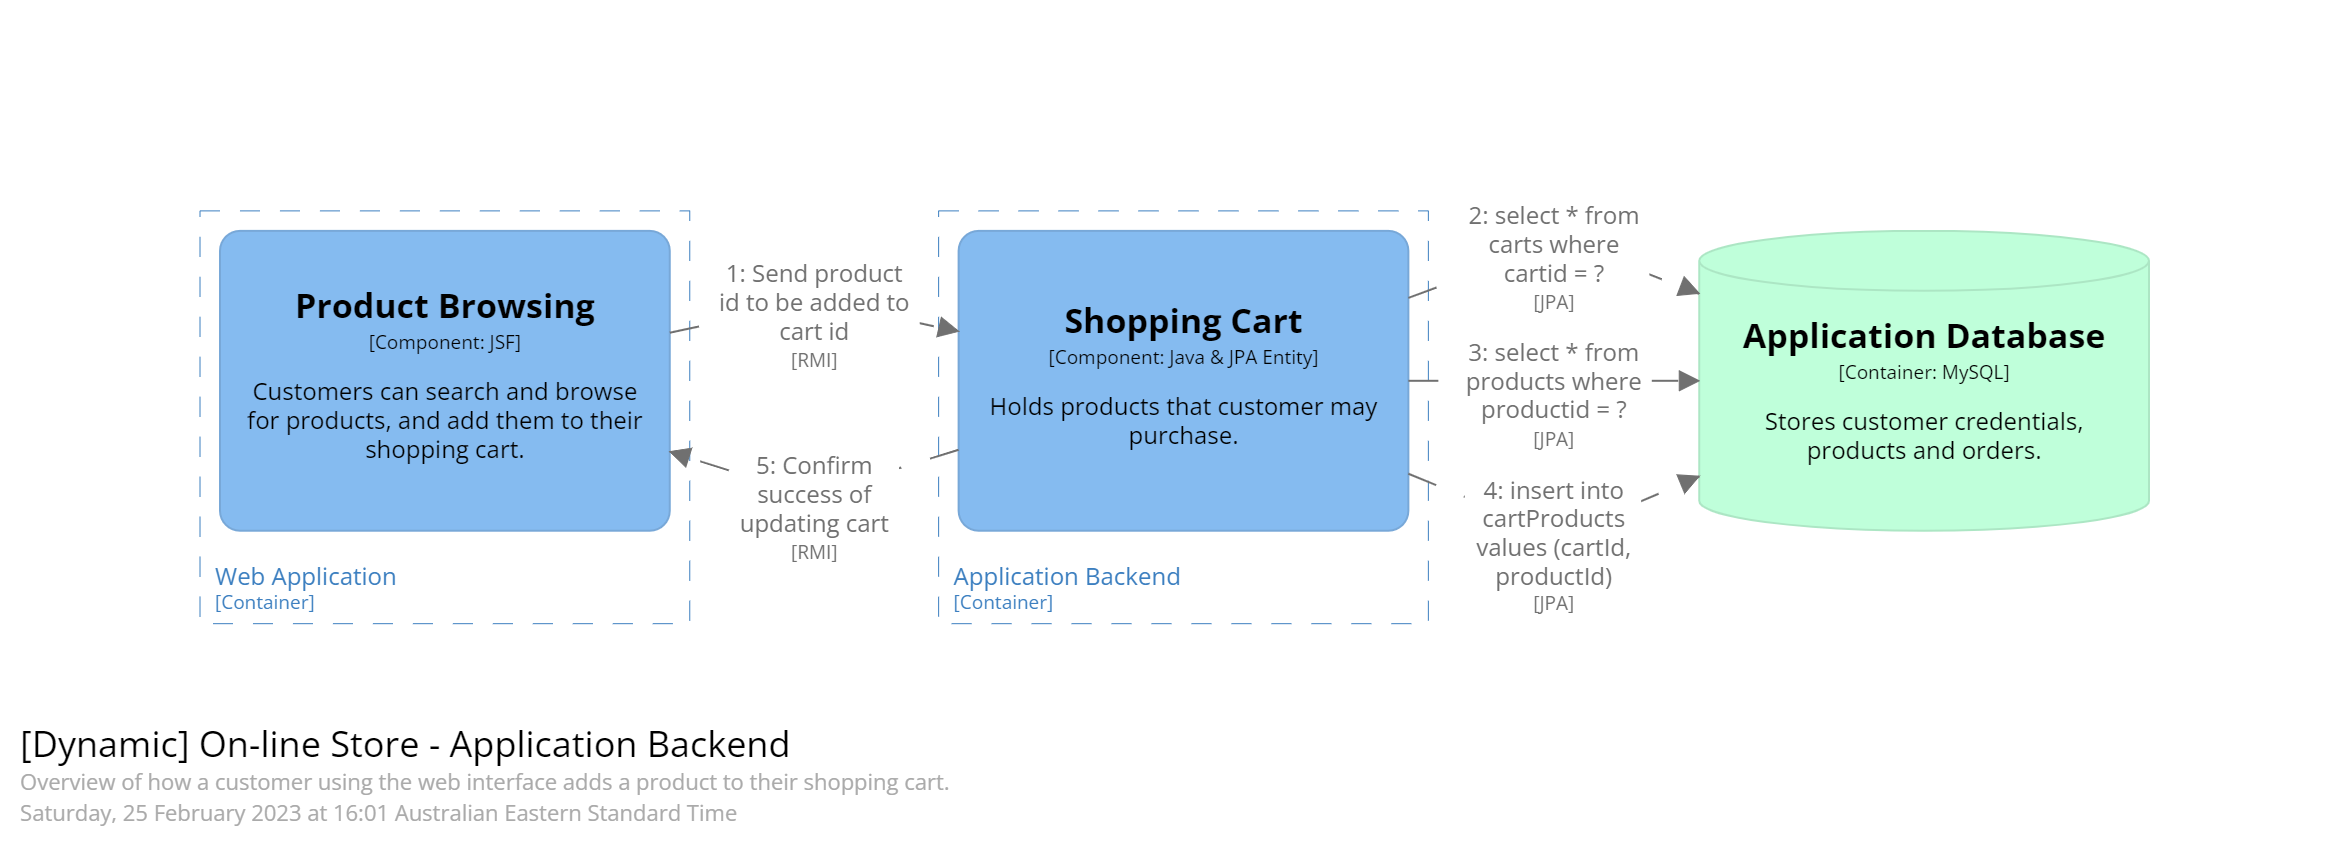
\includegraphics[trim=175 225 197 185,clip,width=\textwidth]{images/c4/add_to_cart_dynamic_diagram.png}
    \caption{Dynamic diagram for adding a product to the customer's shopping cart.}
    \label{fig:c4_dynamic}
\end{figure}

\noindent
If the information is useful, a more detailed dynamic diagram, like the detailed sequence diagram in figure \ref{fig:detailedSequenceDiagram}, can be provided.
Sequence diagrams can be used instead of C4 dynamic diagrams, if the order of events is important.

\subsection{Deployment}\label{sec:c4_deployment}
While not one of the ``four C's'', deployment diagrams are important for most systems.
They describe the physical architecture or infrastructure on which the system will be deployed.
It shows which containers will run on which computing platforms (\emph{deployment nodes}).
Deployment nodes can be nested, as shown in figure \ref{fig:c4_deployment}.
They may also contain infrastructure nodes or software system instances\footnote{\url{https://github.com/structurizr/dsl/blob/master/docs/language-reference.md\#deploymentNode}}.

\begin{figure}[h!]
    \centering
    \begin{adjustwidth}{-7.5mm}{-7.5mm}
        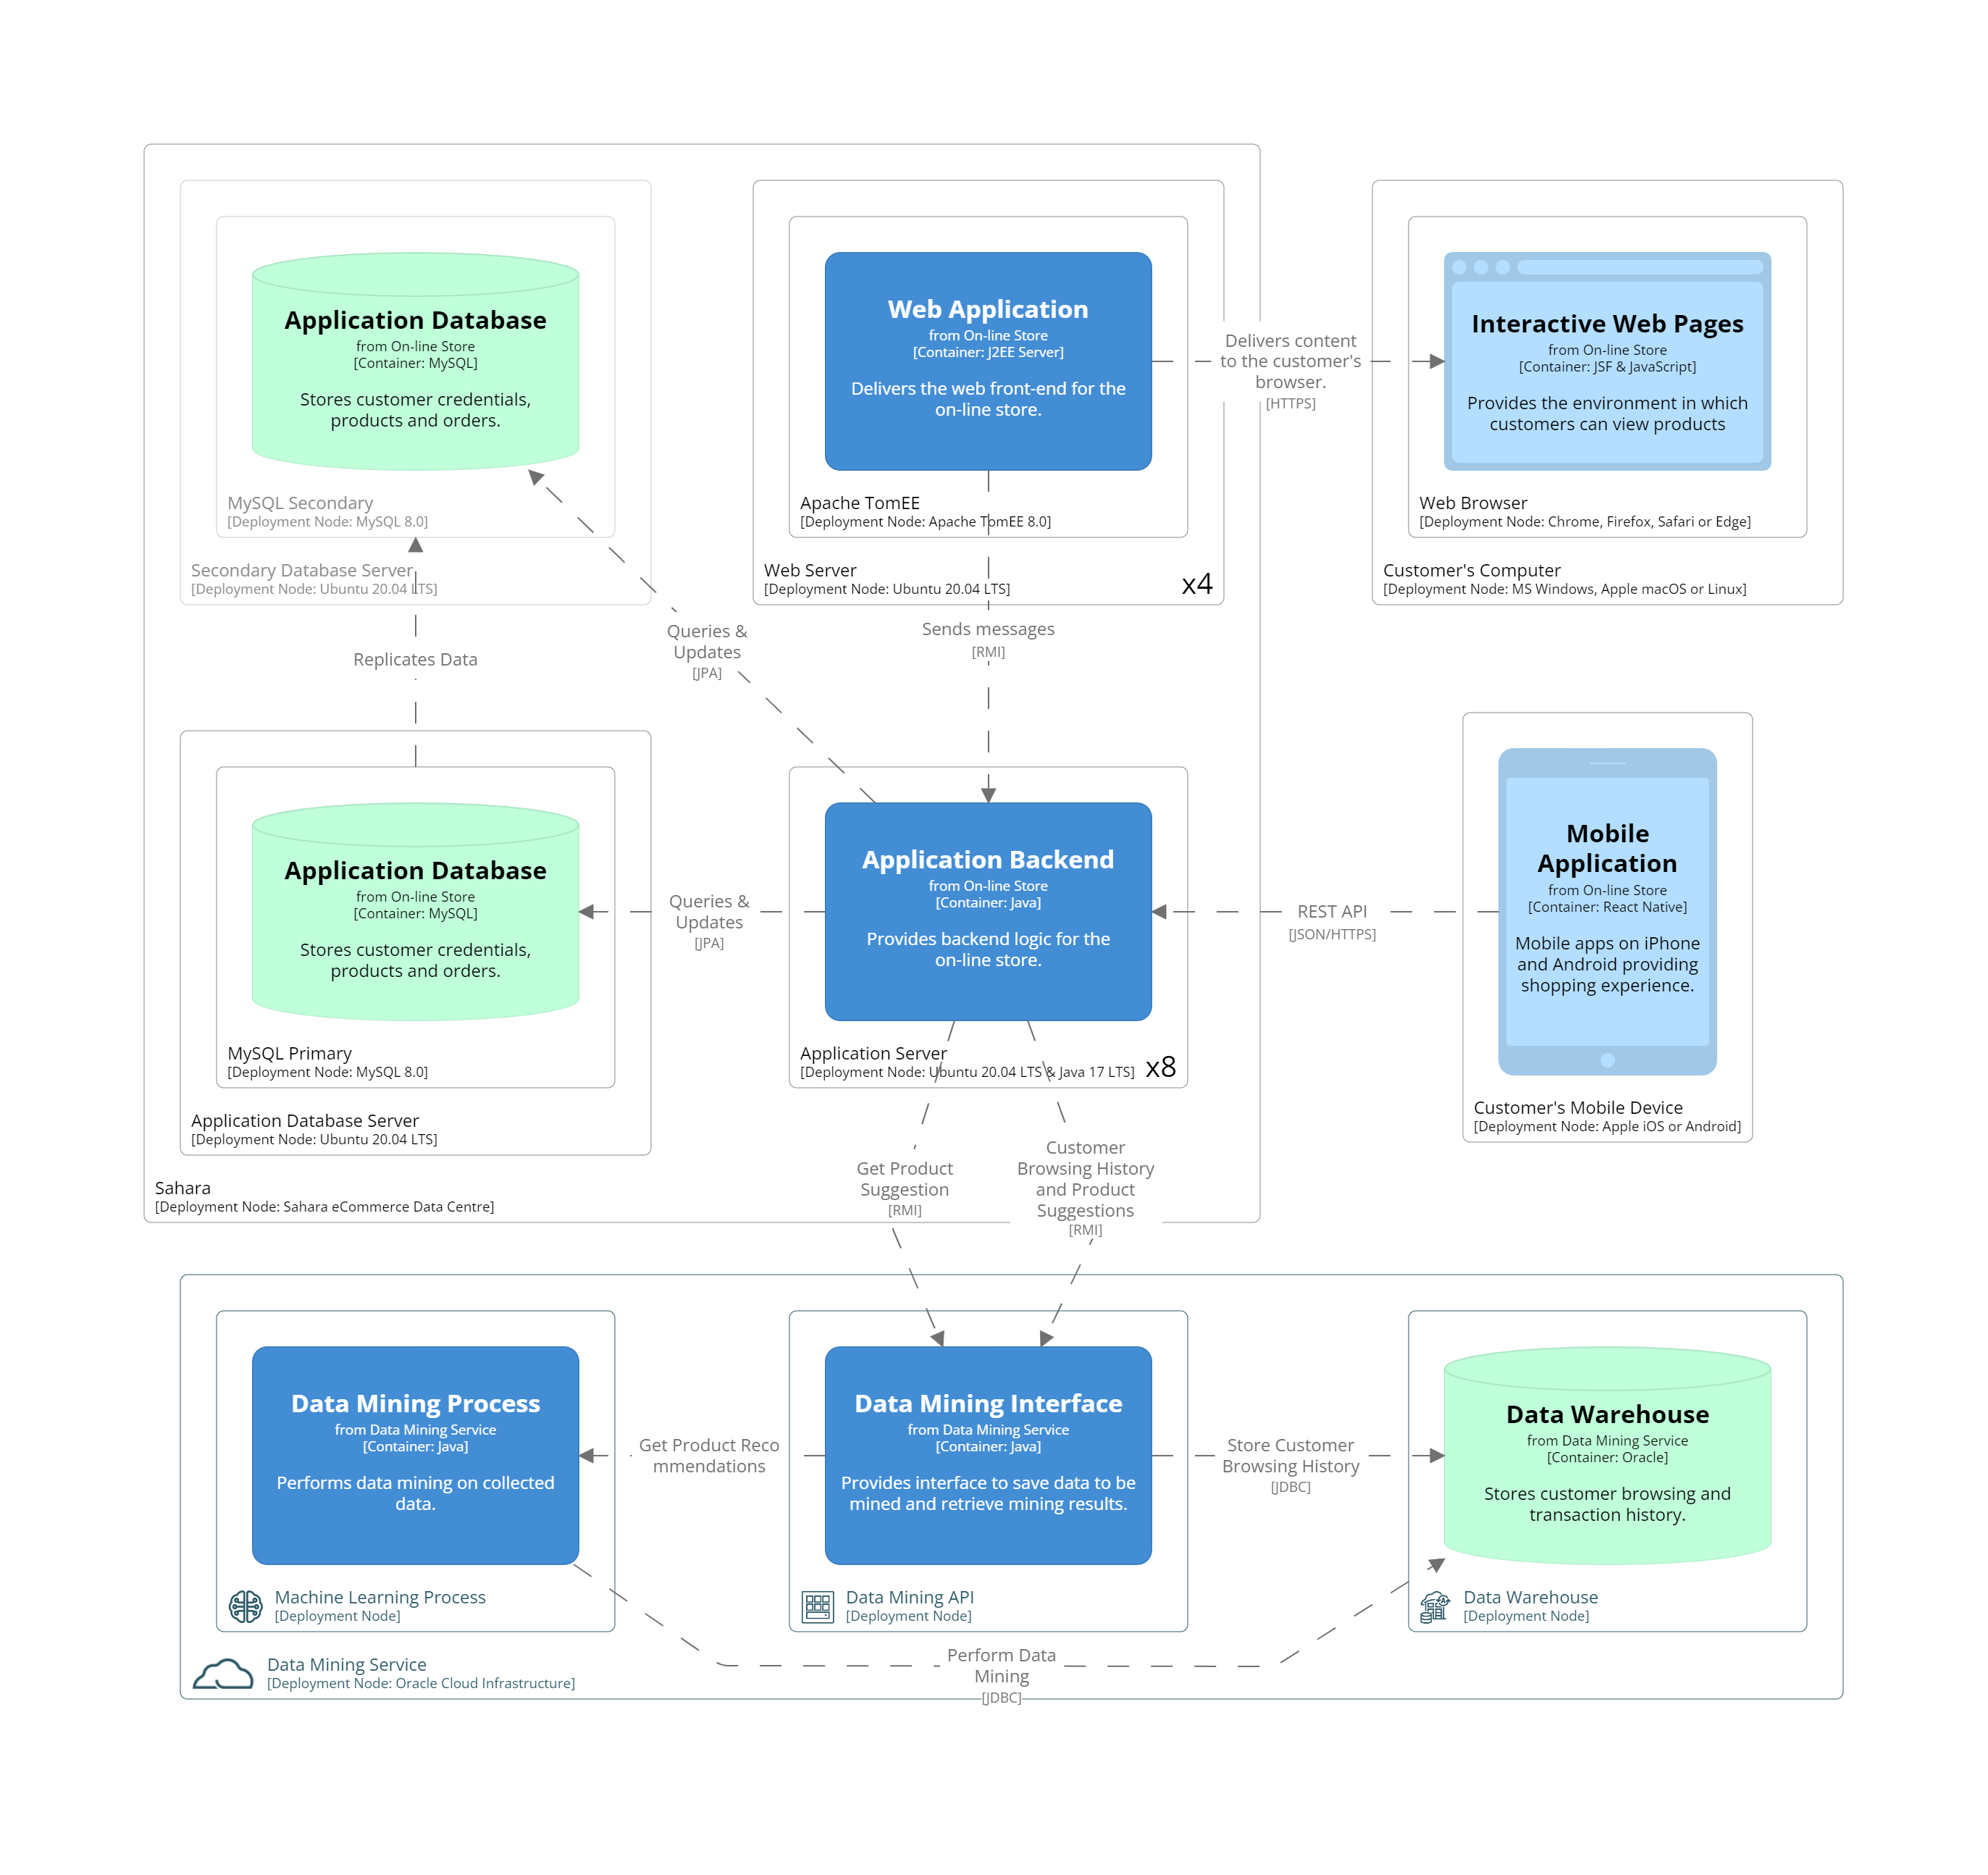
\includegraphics[trim=195 235 195 198,clip,width=0.95\paperwidth]{images/c4/deployment_diagram.png}
    \end{adjustwidth}
    \caption{Deployment diagram for the Sahara eCommerce System.}
    \label{fig:c4_deployment}
\end{figure}

Figure \ref{fig:c4_deployment} is an example C4 deployment diagram for the Sahara eCommerce system.
It takes a slightly different approach to the physical architecture than was shown in figure \ref{fig:deploymentDiagram}.
It shows that the on-line store software system runs in Sahara's data centre.
The data mining service runs on Oracle's cloud infrastructure.
This approach of a system that uses cloud services for some of its implementation is called a \emph{hybrid cloud} application.
There are still the apps running on mobile devices and the code running in the customer's browser.

Like UML, a software environment is embedded in the hardware environment on which it runs.
The web application runs in an Apache TomEE J2EE server, which is running on a Ubuntu server.
The ``\texttt{x4}'' inside the web server deployment node indicates that there will be four of these servers to share the load.
The application backend runs on eight Ubuntu servers, providing the core business logic shared by the web and mobile applications.

The application database runs in MySQL on its own Ubuntu server.
Replication of the application database is explicitly shown in this example, whereas it was not shown in figure \ref{fig:deploymentDiagram}.
Replicating the database running on another server allows for failover.
The application backend can continue to operate if the primary application database fails.

In this version of the example, the application backend communicates with the data mining service
through an API published by the data mining interface running in a virtual machine on Oracle's cloud infrastructure.
The data mining service uses Oracle's machine learning services to perform the data mining.
Oracle's cloud-based data warehouse infrastructure is used to hold all the data.

\noindent
Figure \ref{fig:c4_deployment_key} is the key describing the icons and colours used in the deployment diagram.

\begin{figure}[h!]
    \centering
    \begin{adjustwidth}{-7.5mm}{-7.5mm}
        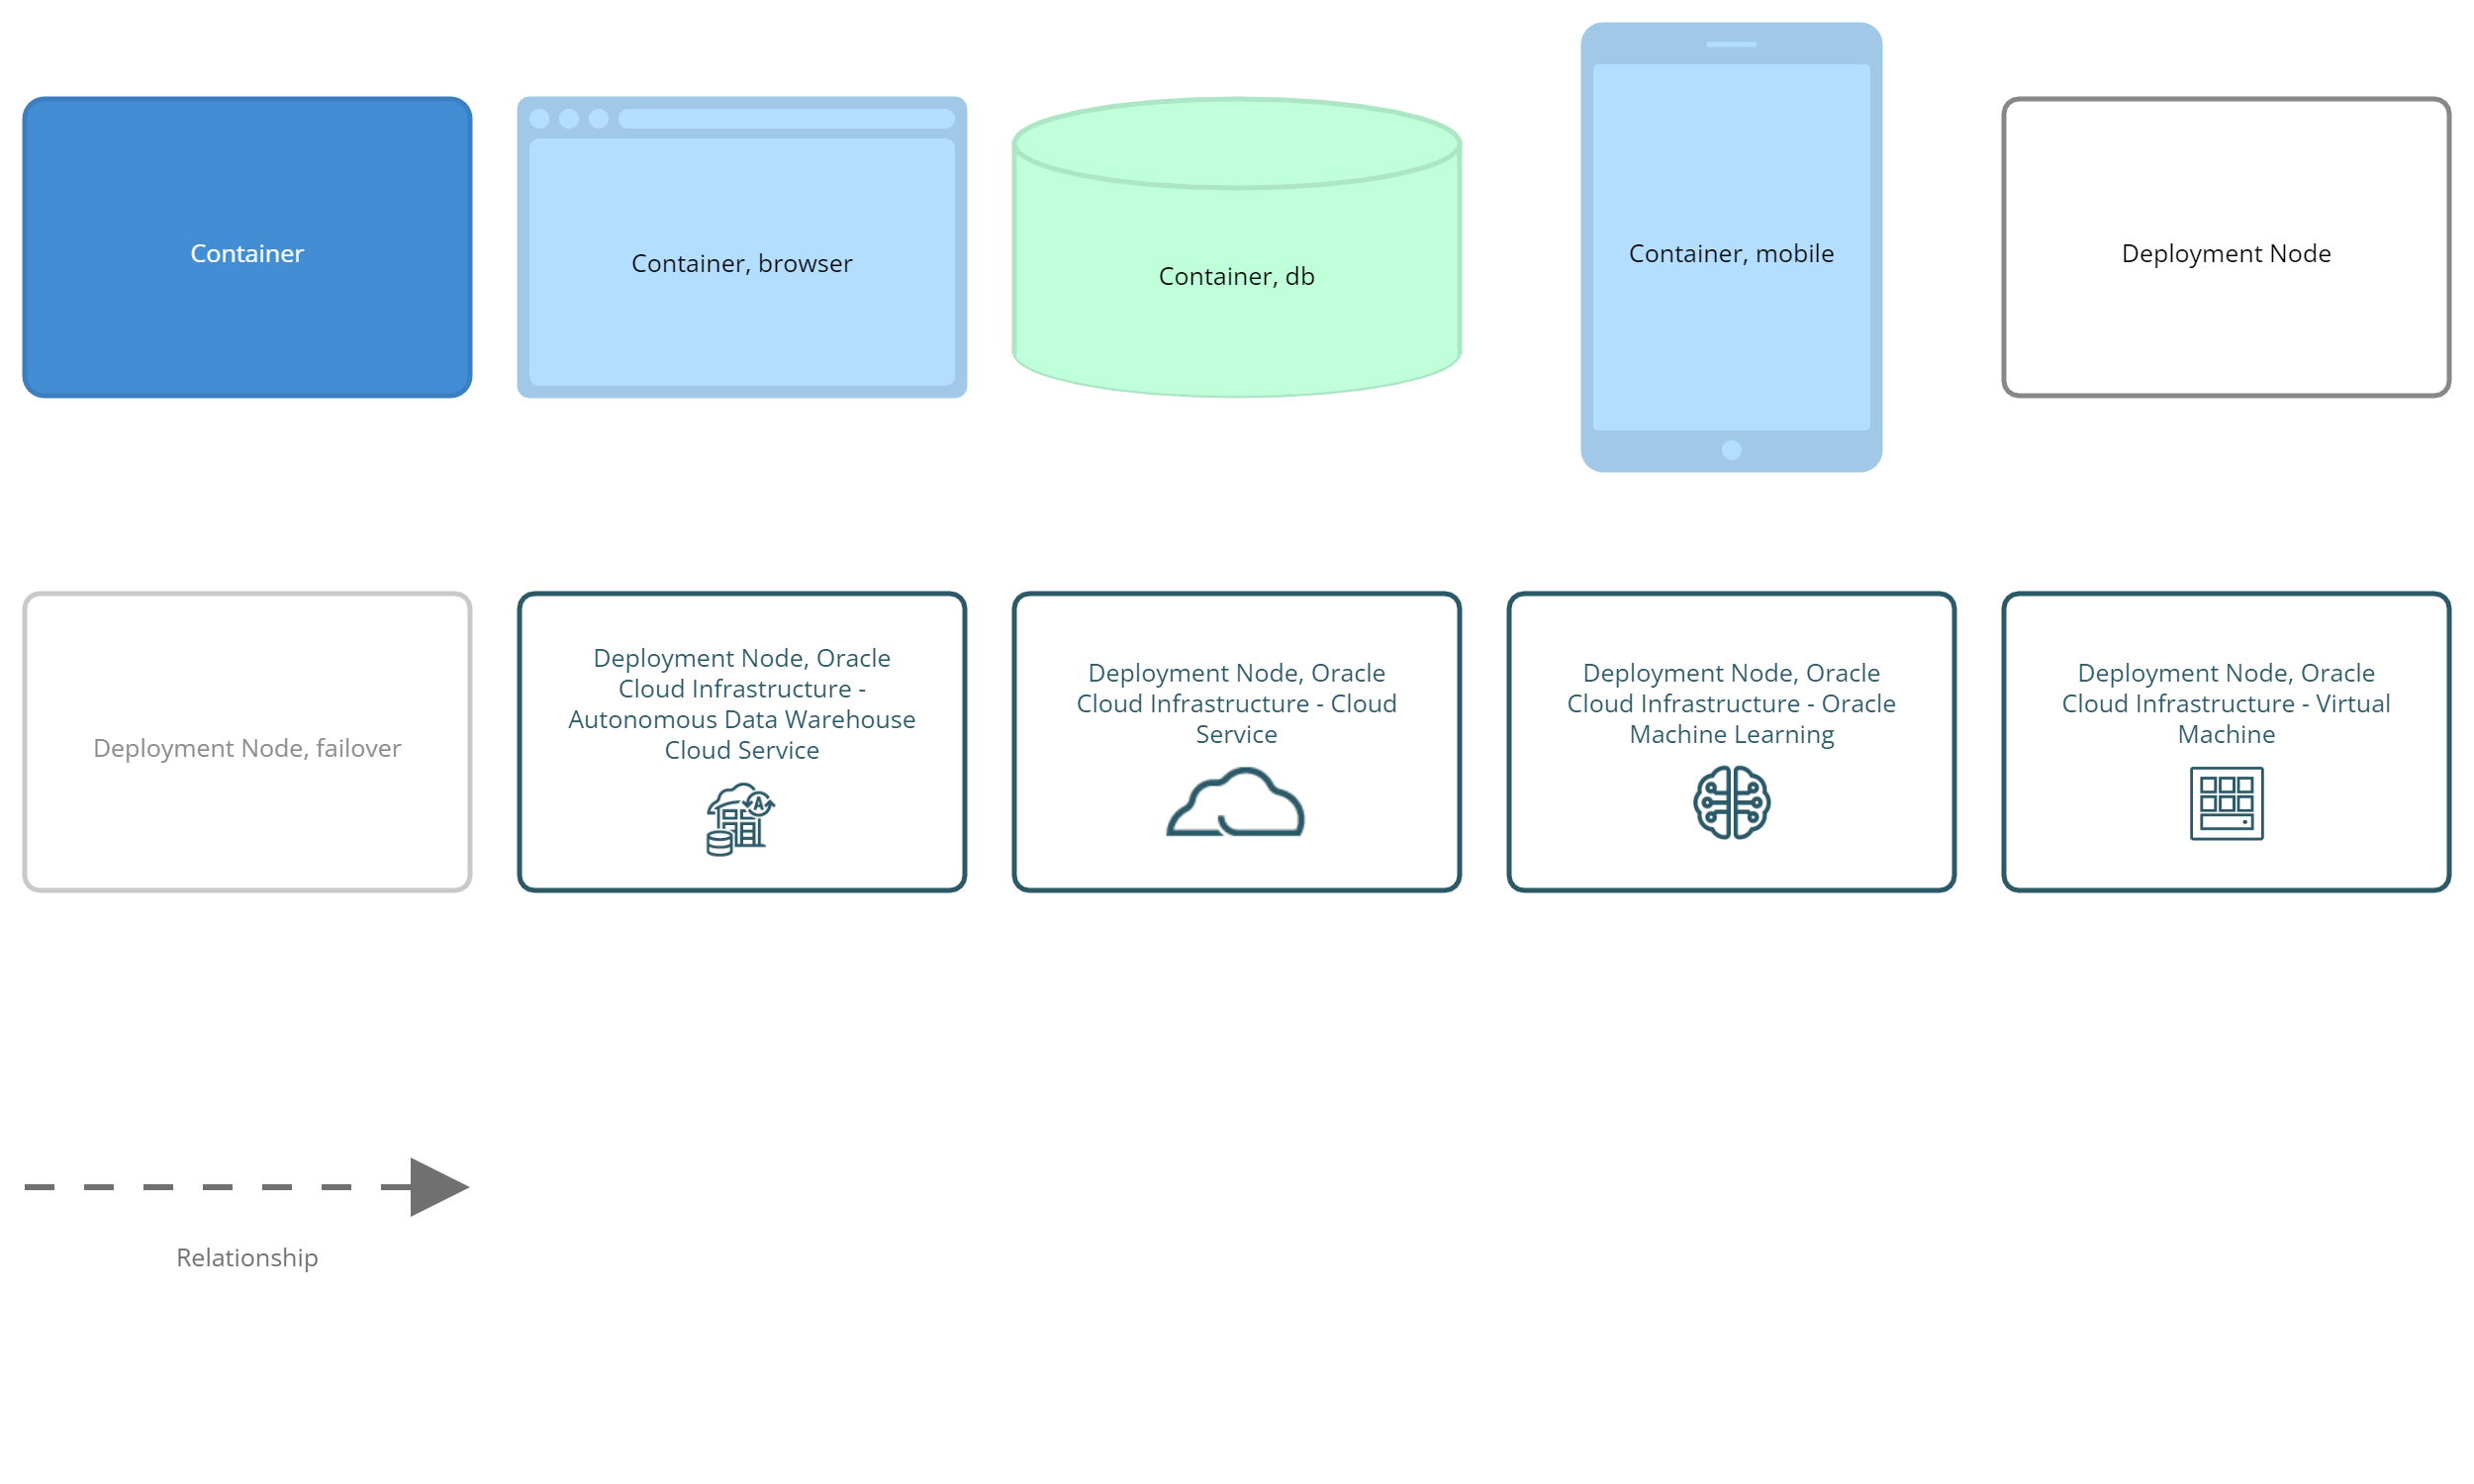
\includegraphics[trim=22 210 22 24,clip,width=0.95\paperwidth]{images/c4/deployment_diagram-key.png}
    \end{adjustwidth}
    \caption{Deployment diagram key.}
    \label{fig:c4_deployment_key}
\end{figure}

\section{Tools}
We do not advocate a specific notation or support tools.
Both UML and C4 have been used so that you are aware of some options.
UML is a standardised notation, with formal syntax and semantics.
There will be situations where the formality will be useful.
C4 is popular because it has a basic structure, but the rules are intentionally loose to make it easy to adopt.

Regardless of whether you use UML, C4 or another notation, you should use tools to aid the creation of your diagrams and documentation.
The important thing is that you want to use a modelling tool, not a drawing tool.
Many drawing tools provide UML templates, and some also support C4.
The issue with drawing tools is that they do not know what the elements of the diagram mean.
If the name of an operation in a class is changed in a drawing tool, you will need to manually change it wherever it is referenced in other diagrams
(e.g. in sequence diagrams).
A modelling tool will track the information that describes the model, so that a change to a model element in one place,
will be replicated wherever that element appears in other diagrams.

There are many tools that support UML.
In a commercial project using UML on a large system, the cost of professional UML tools is negligible and is quickly recovered by the automation they provide.
There are a number of free UML tools. Some to consider are \link{Astah}{https://astah.net/products/free-student-license/},
\link{ModelIO}{https://www.modelio.org/} or \link{PlantUML}{https://plantuml.com/}.
 \begin{description}[nosep]
    \item[Astah] Is a commercial product that supports modelling in many notations. They provide a free UML tool for students.
    \item[ModelIO] Is an open source UML modelling tool.
    \item[PlantUML] Is an open source text-based descriptive language that generates UML diagrams.
                              \link{PlantText}{https://www.planttext.com/} is an online tool supporting it.
\end{description}

\noindent
There are fewer tools that support C4.
\link{Structurizr}{https://www.structurizr.com/} was developed by Simon Brown as a tool to support generating C4 diagrams from textual descriptions.
It is an \link{open source tool}{https://github.com/structurizr/}.
You can use a domain specific language to describe a C4 model, or you can embed the details in Java or .Net code.
There is also \link{C4-PlantUML}{https://github.com/plantuml-stdlib/C4-PlantUML}, which extends PlantUML to support C4.
Astah Professional supports C4, but they no longer provide that version of the tool free to students.

\section{Conclusion}
Architectural views help developers understand different dimensions and details of a complex software architecture.
They are useful both during design and as documentation.
During design, views help you to focus on a particular aspect of the software architecture and ensure that it will allow the system to deliver all of its requirements.
As documentation, views help developers to understand how different aspects of the architecture are intended to behave.

We have intentionally looked at a few different approaches to helping you describe a software architecture.
You should be conversant with multiple different approaches.
The hallmark of a professional is to know when to select a particular approach.

If you compare the ``4+1 View Model'' \cite{4+1-model} with the views described in \textit{Software Architecture in Practice} (SAP) \cite{bass2021software},
you will see that there are obvious similarities but also some differences.
The logical, development and process views from the 4+1 view model map closely to the module and component-and-connector (C\&C) views from SAP.
The physical view corresponds to the allocation view.
The 4+1 view model also includes the scenario view, which does not correspond directly to the SAP views.

The C4 model does not explicitly include the concept of views.
Like SAP, it emphasises the structure of the software architecture.

The scenario view is used to demonstrate how the architecture described in the other views delivers the core functional requirements.
It is used while designing a software architecture to validate that it is suitable for the system.

Kruchten intentionally separated the process view from the logical and development views,
rather than bundling them together like the C\&C view in SAP.
This is because for some systems the dynamic details, which are described by the process view, can be complex and important.
Dealing with issues such as complex concurrency, real-time interactions or latency, can often be more easily considered by having a separate view for them.

Kruchten's experience with Canada's integrated, nation-wide, air traffic control system was such a case.
Data from radar systems and aircraft transponders have to be processed and reported to air traffic controllers in near real-time.
With thousands of input sources and hundreds of controller stations, understanding concurrency issues is critical.
Tracking aircraft from one control space to another means that communication latency is important.
Each control space has its own hardware and is separated from neighbouring spaces by hundreds or thousands of kilometres.

As a software architect you need to choose which views provide meaningful information about your software system.
The graphical notation used to describe a view is only one part of the view (though an important part).
Ensure you provide enough supporting information so others will know how to work with your architecture and why you made the choices that you did.